\documentclass{iiuwb}
\usepackage[polish]{babel}
\usepackage{enumerate}
\usepackage{graphicx}
\usepackage{indentfirst}
\usepackage{listings}

\usepackage{epstopdf}    % for automatic conversion from eps files to pdf
\usepackage{hyperref}   % do~tworzenia linków zewnętrznych \url{...} oraz wewnętrznych
\usepackage[normalem]{ulem}  %strikethrough

\renewcommand{\imiona}{Mateusz}
\renewcommand{\nazwiska}{Wróblewski}

\renewcommand{\stopienpromotora}{dr inż.}
\renewcommand{\imionapromotora}{Andrzej}
\renewcommand{\nazwiskapromotora}{Kużelewski}

%\renewcommand{\profuwb}{TAK}
\renewcommand{\profuwb}{NIE}

%W przypadku braku asystenta pozostawić PUSTE
\renewcommand{\stopienasystenta}{}
\renewcommand{\imionaasystenta}{}
\renewcommand{\nazwiskaasystenta}{}

\renewcommand{\tytul}{Analiza porównawcza narzędzi do orkiestracji kontenerów Docker}
\renewcommand{\rok}{2023/2024}
\renewcommand{\zaklad}{Sztucznej Inteligencji i~Multimediów}
\renewcommand{\album}{12321}
\renewcommand{\rokakademicki}{2020/2021}
\renewcommand{\kierunek}{Informatyka}

%Wybrać ścieżkę
%\renewcommand{\sciezka}{Grafika}
\renewcommand{\sciezka}{\dotfill}


%%% Wybrać właściwy
\renewcommand{\rodzaj}{stacjonarne}
%\renewcommand{\rodzaj}{niestacjonarne}


%%% Wybrać właściwy
%\renewcommand{\poziom}{magisterskie jednolite}
%\renewcommand{\poziom}{magisterskie uzupełniające}
% \renewcommand{\poziom}{I stopnia}
\renewcommand{\poziom}{II stopnia}

\begin{document}
%Spis treści
\tableofcontents

% Właściwa zawartość

\cleardoublepage
\chapter*{Wstęp}                %rozdział nienumerowany
\label{cha:Wstep}                       %w \label nie~używamy polskich znaków
\addcontentsline{toc}{chapter}{Wstęp}   %dorzucamy ręcznie do~spisu treści

Obecnie zauważalny jest trend przejściowy z dużych monolitycznych 
aplikacji, na aplikacje mikroserwisowe. Jak dotąd powszechnie 
powstawały duże i ciężkie aplikacje, lecz w powodu powstania 
\textit{Dockera} i \textit{orkiestratorów} coraz częściej zaczęto przechodzić na 
podział tej aplikacji na mniejsze części.

Aplikacje \textit{monolityczne} polegają na jednoczesnym uruchomieniu 
wszystkich komponentów aplikacji w tym samym czasie. Co za tym 
idzie zmiany w jednym komponencie wymagają restartowania całości.

Z drugiej strony aplikacje \textit{mikroserwisowe} polegają na podziale 
serwisu na mniejsze niezależne części, które komunikują się za 
pośrednictwem \textit{API}. Pozwala to na podział obowiązków między 
członkami zespołu w taki sposób, żeby praca jednej osoby nie 
wpływała na pracę drugiej. Co prowadzi do zwiększenie 
elastyczności i ułatwia utrzymanie kodu aplikacji.

\begin{table}[!h]
\caption{Wady i zalety aplikacji Monolitycznych i mikroserwisowych}
\begin{center}
\begin{tabular}{| p{5cm} | p{5cm} |}
\hline
Aplikacje monolityczne  & Aplikacje mikroserwisowe\\
\hline
\hline
Może wystąpić problem w dodaniu nowych technologii do projektu &
 Pozwala na stopniowe przepisywanie części na kodu na nowe 
technologie   \\ \hline
Proste do implementacji & 
Wszystkie komponenty są tworzone oddzielnie co pozwala na lepsze 
ich skalowanie i możliwość osiągnięcia lepszej wydajności \\ \hline
Potrzeba więcej czasu na dodanie nowych funkcjonalności &
 Trudne testowanie wszystkich serwisów \\ \hline
Poszczególne elementy systemu są zależne od siebie, co powoduje 
pojawienie się błędu w innej części aplikacji po wprowadzeniu 
zmian & Potrzebna jest dodatkowa infrastruktura, która pomoże 
obsłużyć wszystkie komponenty aplikacji np. AWS \\ \hline
Mniejsza skalowalność niż w przypadku aplikacji mikroserwisowych & 
Serwisy są odizolowane co sprawia, że pojawienie się błędu w 
jednym serwisie, nie będzie mieć on wpływu na cały system. \\ \hline
Szybsza komunikacja między komponentami & Wydajność całej aplikacji może być niska z powodu opóźnień w komunikacji między serwisami. \\ \hline
Łatwe do zarządzania i monitorowania  & Tworzenie aplikacji mikroserwisowej wymaga dużej wiedzy i umiejętności. \\ \hline
\end{tabular}
\label{tab:Wady i zalety aplikacji Monolitycznych i mikroserwisowych}
\end{center}
\end{table}

Popularnym narzędziem do tworzenia aplikacji mikroserwisowych jest 
\textit{Docker} \ref{cha:Konteneryzacja}. Pozwala on odizolować i podzielić 
poszczególne części aplikacji, na elementy zwane \textit{kontenerami}. 
Każdy \textit{kontener} posiada wszystko co potrzebuje, aby zostać 
uruchomiony, więc  bez znaczenia, gdzie będzie uruchomiony, będzie 
działał zawsze tak samo. Pozwala to programistom na wybór odnośnie 
używanego systemu operacyjnego. Ponadto kontenery są łatwo 
skalowalne i nie wymagają dużych mocy obliczeniowych w odróżnieniu 
do maszyn wirtualnych.

W pewnym momencie rozwoju aplikacji, gdy aplikacja staje się coraz większa. Przychodzi problem związany z zarządzaniem wszystkimi kontenerami. Z pomocą przychodzą narzędzia zwane \textit{orkiestratorami}, za pomocą których można zarządzać całym cyklem życia \textit{kontenerów}, czyli wdrażaniem, aktualizowaniem, skalowaniem i usuwaniem. Przykładowymi zadaniami orkiestatorów jest dynamiczne przypisanie zasobów, monitorowanie wydajności kontenerów, czy odbudowa kontenera w przypadku wystąpienia błędów. W rozdziale \ref{cha:Orkiestratory} zostały opisane wykorzystane orkiestatory.

Aspektem teoretycznym pracy jest zapoznanie się z narzędziem Docker\ref{cha:Konteneryzacja}, jego możliwościami, komendami i sposobem działania. Następnie zaprojektowanie aplikacji\ref{cha:Aplikacja} za pomocą której będzie można porównać dane \textit{orkiestratory} opisane w rozdziale \ref{cha:Orkiestratory}.

Aspekt praktyczny składa się z własnoręcznego zaimplementowania aplikacji i jej skonteneryzowania. Następnie zainstalowania i skonfigurowania \textit{orkiestratorów} lokalnie, a na koniec wykonanie testów, takich jak sprawdzenie obiążenia podzespołów, czasu uruchomienia, czy sprawdzenie wytrzymałości na ruch użytkowników, poprzez zalanie aplikacji dużą ilością zapytań. Teoretycznie najlepsze wyniki powinny wyjść dla Docker Swarma, ponieważ jest to wewnętrzne narzędzie Dockera do okrkiestracji kontenerów. Jest również najmniej rozbudowane i ma najmniej funkcji. Wyniki dla Kubernetesa i Nomada powinny być zbliżone. Są to narzędzia, które wymagają dodatkowego oprogramowania i odpowiedniego zkonfigurowania.

Po wstępnej analizie dostępych narzędzi, został wybrany framework Quarkus\ref{sec:Quarkus} z powodu dużego wsparcia dla Kubernetesa \ref{sec: Kubernetes} i konteneryzacji. Jak i również sprawdzenia, czy rzeczywiście uzyskam lepsze dla niego lepsze wyniki w porównanie z innymi okiestratorami. Podczas testów startu aplikacji, czy podczas testowania ruchu w aplikacji będą wysyłane zapytania do stworzonego API i na podstawie odpowiedzi, będzie można wyciągnąć odpowiednie wnioski.
\newline

Cała praca składa się z pięciu rozdziałów. W rozdziale \ref{cha:Konteneryzacja} jest przedstawiona 
historia konteneryzacji, jej zalety oraz wady. Następnie opisane są podstawowe elementy potrzebne do 
korzystania z Dockera. Na koniec jest porównianie z innym równie popularnym narzędziem do 
\textit{orkiestracji}, czyli Podmanem. \ref{cha:Aplikacja} rozdział został poświęciony informacjom o aplikacji. 
Co ta aplikacja ma robić i jakie technologie zostały użyte do jej wykonania. \ref{cha:Orkiestratory} rozdział 
będzie mówił o orkiestacji. Przedstawiony zostanie opis poszczególnych \textit{orkiestratorów}: Docker Swarm, 
Kubernetes oraz Nomad. Omówione zostaną architektury systemu dla każdego orkiestatora oraz w jaki sposób 
serwisy się łączą. ref{cha:Opis eksperymentów} rozdział przedstawia platformę testową oraz użyte narzędzia 
do testowania i sposób ich wykorzystania. Ostatni \ref{cha:Analiza Wynikow} rozdział przedstawia uzyskane 
wyniki oraz ich interpetację.

%%%%%%%%%%%%%%%%%%%%%%%%%%%%%%%%
\cleardoublepage
\chapter{Konteneryzacja}
\label{cha:Konteneryzacja}

Za pierwsze początki konteneryzacji można uznać rok 1979. W tym roku wynaleziono operację chroot. Jest to operacja dostępna w systemach unixowych. Umożliwia ona utworzenie środowiska, które jest odizolowane od systemu plików gospodarza. Nie można odczytać folderów, ani plików, które nie należą do utworzonego środowiska. Do utworzonego procesu można przypisać zasoby, takie jak moc procesora, ilość pamięci operacyjnej, czy pojemność dysku ssd.

\section{Podstawowe pojęcia konteneryzacji za pomocą Dockera}

W ręcznym budowaniu odizolowanego środowiska występuje problem w przypadku wprowadzania zmian. W takim przypadku należy wszystko od początku instalować i uruchamiać. Z pomocą przychodzi Docker za pomocą, którego z łatwością uruchomimy kontener z aplikacją. 

\subsection{Plik konfiguracyjny Dockerfile}
\label{sec:dockerfile}

Plik DockerFile jest to plik tekstowy, który zawiera listę komend do utworzenia obrazu\ref{images and containers}.

Pierwszą komendą jaka musi wystąpić w pliku jest \textbf{FROM}, która jest referencją do istniejącego obrazu. Jest to podstawa budowy całego obrazu, np. \textbf{FROM NGINX} oznacza, że obraz będzie zbudowany na podstawie obrazu serwera NGINX.

Drugą komendą jest \textbf{COPY} za pomocą, której kopuje się pliki z systemu gospodarza do odizolowanego środowiska.

Trzecią komendą jest \textbf{ENV}, która określa zmienne środowiskowe według wzoru <klucz>=<wartość>.

Ostatnimi komendami są \textbf{EXPOSE} do ustalenia portu pod jakim będzie można połączyć się z aplikacją oraz \textbf{USER} do ustanowienia nazwy użytkownika.\newline

Przykładowy plik \textbf{Docker File}\newline

\begin{lstlisting}[breaklines=true]

FROM registry.access.redhat.com/ubi8/openjdk-17:1.16

ENV LANGUAGE='en\_US:en'

COPY --chown=185 target/quarkus-app/lib/ /deployments/lib/
COPY --chown=185 target/quarkus-app/*.jar /deployments/
COPY --chown=185 target/quarkus-app/app/ /deployments/app/
COPY --chown=185 target/quarkus-app/quarkus/ /deployments/quarkus/

EXPOSE 8080
USER 185

ENV JAVA\_OPTS="-Dquarkus.http.host=0.0.0.0 -
Djava.util.logging.manager=org.jboss.logmanager.LogManager"
ENV JAVA\_APP\_JAR="/deployments/quarkus-run.jar"

\end{lstlisting}

\subsection{Obrazy i kontenery Dockerowe}
\label{images and containers}

Docker pozwala na spakowanie aplikacji i uruchomienie jej w kontenerze. Operacja ta działa na każdym systemie opercyjnym umożliwiającym wirtualizacje w którym zainstalowany jest Docker.

Kontener Dockerowy jest to środowisko uruchomieniowe ze wszystkimi zależnościami, jak kod programu czy biblioteki. Aby utworzyć kontener potrzebny jest obraz. Warstwy utworzone przy pomocy obrazu są niemodyfikowalne, ale jest możliwość zainstalowania na najwyższej warstwie swojej aplikacji czy utworzenie własnych zmiennych i dodanie danych. W celu efektywnego zarządzania dużą ilością kontenerów potrzebne jest narzędzie zwane \textit{orkiestratorem} \ref{cha:Orkiestratory}. 
\newline
Najbardziej przydatne komendy w przypadku kontenerów to:
\begin{description}
  \item[docker container run] -- tworzy i uruchamia kontener wykorzystując obraz,
  \item[docker container logs] -- pozwala przejrzeć logi kontenera,
  \item[docker ps] -- wyświetla listę aktualnie uruchomionych kontenerów, po dodaniu parametru -a wyświetla również zatrzymane kontenery,
  \item[docker start] -- uruchamia kontener,
  \item[docker stop] -- zatrzymuje kontener,
\end{description}
Wszystkie komendy można zobaczycć w dokumentacji dostępnej pod liniem \newline
\url{https://docs.docker.com/reference/cli/docker/container/}.
\newline

Obraz Dockerowy jest to niezależny, uruchamialny plik używany do stworzenia kontenera. Do jego stworzenia potrzebny jest kod aplikacji, wszystkie zależności, biblioteki oraz Dockerfile \ref{sec:dockerfile}. Służy głównie do przechowywanie konfiguracji aplikacji jako szablon i można go udostępnić dla innych osób, żeby mogli go zainstalować na własnym systemie. Można także wzdrożyc go na publiczne repozytorium, takie jak Docker Hub. Obrazem może być system operacyjny lub baza danych. Nie da się danego obrazu modyfikować jak już został utworzony.
\newline
Najbardziej przydatne komendy w przypadku obrazów to:
\begin{description}
  \item[docker images] -- wypisuje listę dostępnych lokalnie obrazów,
  \item[docker create] -- tworzy obraz, wraz z utworzenie kontenera, ale bez uruchomienia go,
  \item[docker run] -- tworzy obraz, wraz z utworzenie kontenere i jego uruchomieniem
  \item[docker pull] -- ściąga obraz ze zdalnego repozytorium
\end{description}
Wszystkie komendy można zobaczycć w dokumentacji dostępnej pod linkiem \newline
\url{https://docs.docker.com/reference/cli/docker/image/}.
\newline

Przykładowe komendy pozwalające zbudować aplikację opisaną w rozdziale \ref{cha:Aplikacja}.

\begin{itemize}
    \item ,,\textbf{./mvnw package}'' - przed zbudowaniem obrazu, należy zbudować cała aplikację za pomocą \textbf{Mavena}, 
    \item ,,\textbf{docker build -f src/main/docker/Dockerfile.jvm -t APP-NAME .}'' - komenda budująca obraz przy użyciu pliku Dockerfile, 
    \item ,,\textbf{docker run -i --rm -p 8080:8080 APP-NAME}'' -  uruchomienie kontenera na podstawie zbudowanego obrazu, 
\end{itemize}

\section{Różnica między konteneryzacją, a writualizacją}

Wirtualizacja jest to proces tworzenia wartstwy między systemem hosta, a maszyną wirtualną. Komputer zostaje podzielony na wiele mniejszych wirtualnych systemów, gdzie każdy z nich ma swój własny system operacyjny, zasoby i każdy z nich działa niezależnie. Oprogramowanien, które umożliwia wykonanie wirtualizacji jest hypervisor.

W przypadku konteneryzacji, nie tworzy się osobnego systemu od początku, ale używane są zasoby i system operacyjny hosta. Do tego wykorzystywane jest specjalne oprogramowanie do konteneryzacji, jak Docker albo Podman.

Przykładowy pogląd na oba przypadki przedstawiłem na rysunku \ref{fig: Konteneryzacja i wirtualizacja}

\begin{figure}[!h]
\centering
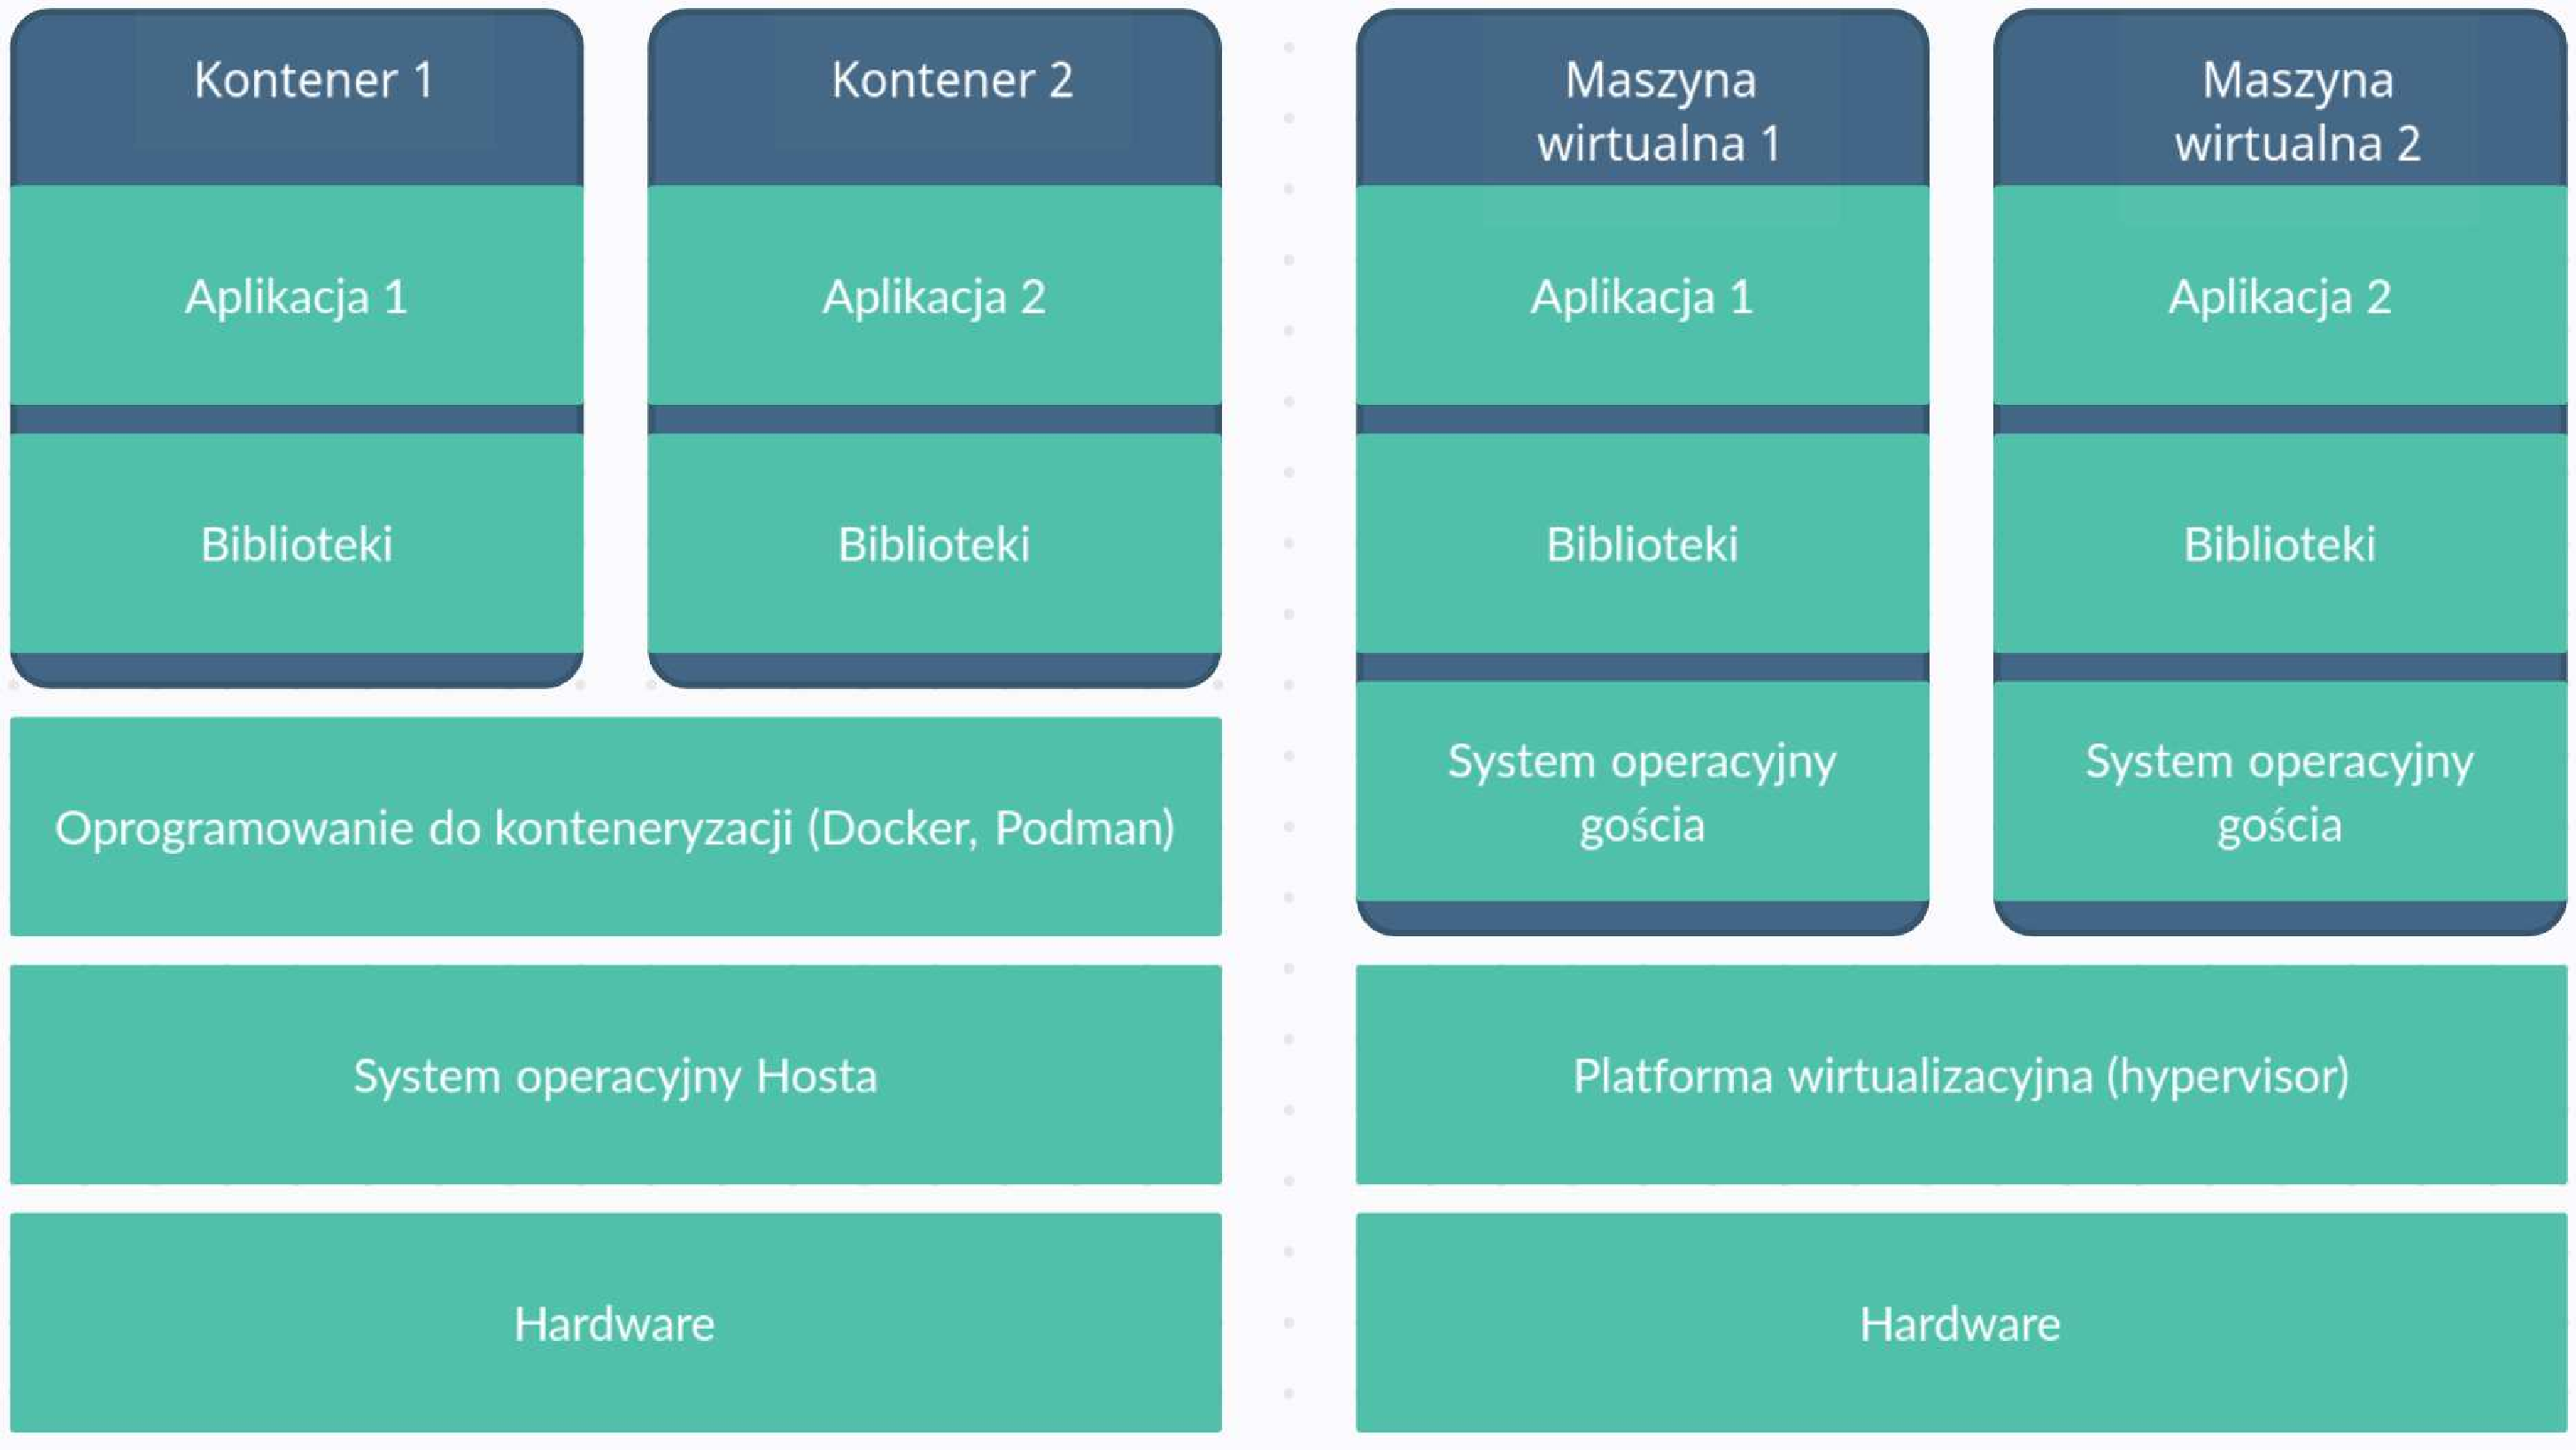
\includegraphics[width=12cm]{kontenery_wirtualizacja.pdf}
\caption{konteneryzacją i wirtualizacją}
\label{fig: Konteneryzacja i wirtualizacja}
\end{figure}

\begin{table}[!h]
\caption{Różnice między wirtualizacją, a konteneryzacją}
\begin{center}
\begin{tabular}{| c |  p{5cm} | p{5cm} |}
\hline
Cecha  & Konteneryzacja & Wirtualizacja\\
\hline
\hline
Użyte zasoby & W powodu używania systemu operacyjnego hosta potrzebują mało zasobów do działania. & Każda maszyna wirtualna korzysta z własnego systemu operacyjnego, więc do stworzenia wielu takich maszyn potrzebne jest wiele zasobów. \\ \hline
Czas uruchomienia & Kontenery szybciej się uruchamiają, ponieważ nie potrzebują uruchamiać całego systemu. & Maszyny wirtualne potrzebują dużo czasu do uruchomienia.\\ \hline
Izolacja & Kontenery używają zasoby sprzętowe hosta, więc w przypadku wystąpienia luk w zabezpieczeniach kontenera może to być wykorzystane przez osoby trzecie. & Maszyny wirtualne działają niezależnie. Błędy i luki, które mogą wystąpić w jednej maszynie wirtualnej nie mają wpływu na działanie innej maszyny wirtualnej.\\ \hline
Łatwość i szybkość użycia & Kontenery można łatwo i szybko tworzyć i uswać.  & Maszyny wirtualne potrzebują, więcej czasu na uruchomienie oraz wymagają ich odpowiedniego zkonfigurowania.  \\ \hline
Ilość potrzebnego miejsca & Obrazy Dockerowe są małe. Jeden obraz zajmuje jednostkę rzędu MB danych.  & Maszyny wirtualne potrzebują, więcej miejsca, gdyż jedna maszyna wirtualna zajmuje jednostkę rzędu GB danych.  \\ \hline
Kompatybilność & Kompatybilne tylko z dystrybucjami Linuxa. Narzędzia takie jak \textbf{Docker Desktop} umożliwiają działanie na \textbf{Windowsie} i \textbf{MacOS} & Maszyny wirtualne są kompatybilne ze wszystkimi systemami operacyjnymi. \\ 
\hline
\end{tabular}
\label{tab:Różnice między konteneryzacją, a wirtualizacją}
\end{center}
\end{table}

\section{Docker i Podman}

Podman jest narzędziem Open Source stworzonym przez firmę Red Hat. Podobnie jak Docker służy do tworzenia i zarządzania kontenerami. W tej sekcji przedstawię różnice i podobienśtwa między tymi narzędziami.

\begin{figure}[!h]
\centering
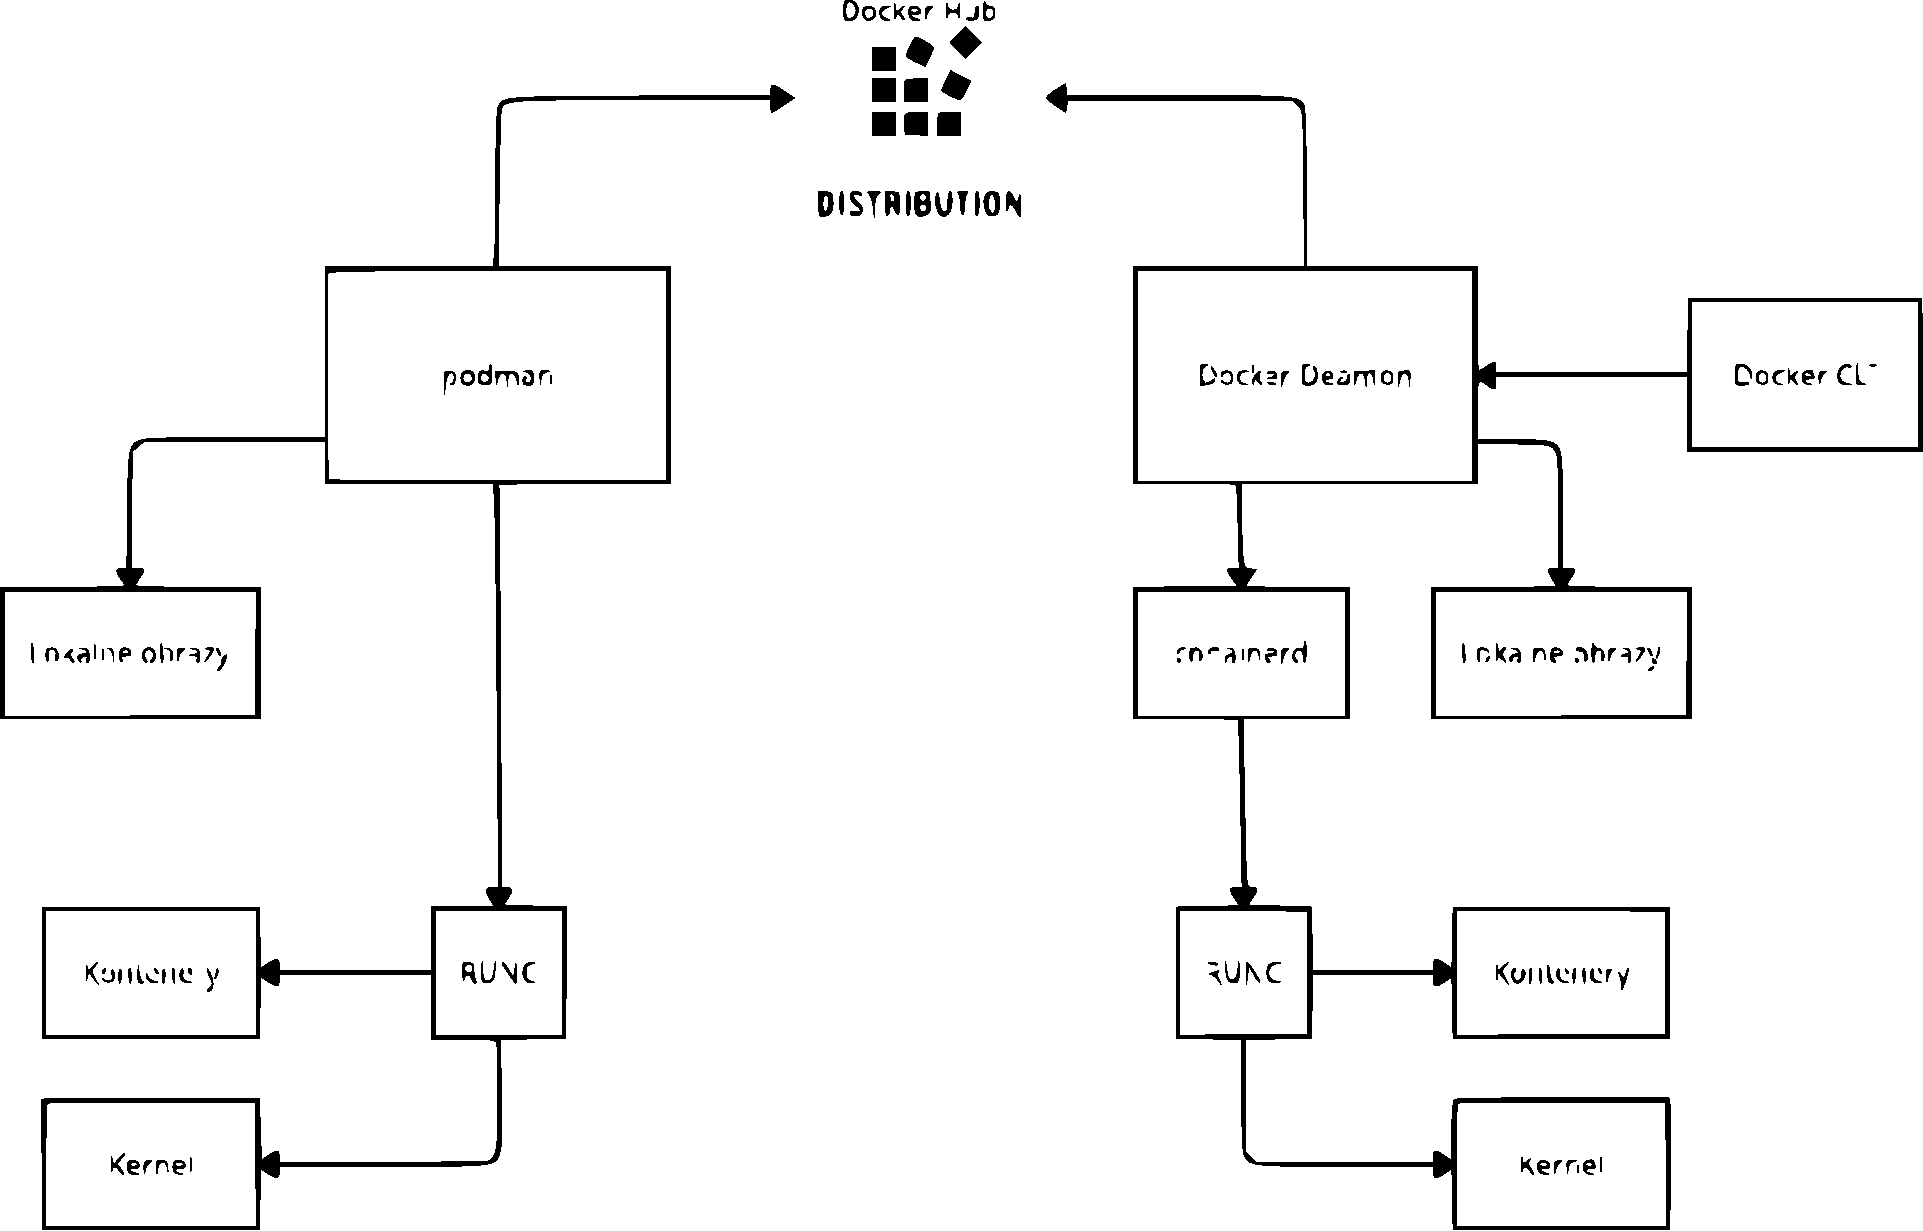
\includegraphics[width=12cm]{ArchitekturaDockeriPodman.pdf}
\caption{Architektura Dockera i Podmana}
\label{fig: Architektura Dockera i Podmana}
\end{figure}

Architektura Dockera jest architekturą 
typu klient-serwer, gdzie użytkownicy komunikują się z Docker daemonem, 
który jest odpowiedzalny za budowanie, uruchamianie i dystrybucję kontenerów. Komunikacja odbywa się 
za pomocą REST API przy pomocy Docker CLI. Podman za to nie posiada własnego deamona. Obsługa i zarządzanie 
kontenerami odbywa się bezpośrednio przez Podman CLI. Co przekłada się na szybkość poleceń. Obie architektury 
zostały przedstawione razem na rysunku \ref{fig: Architektura Dockera i Podmana}. \newline

Polecenia -- treść i zachowanie poleceń są bardzo podobne, zwykle jedyną różnicą jest zamiana słowa kluczowego docker na podman. W poniższym przykładzie przedstawiłem dwie komendy, które tworzą kontener z systemem nginx: 

\noindent -- \textbf{podman run --name mynginx1 -dt -p 8080:80/tcp docker.io/nginx} \newline
-- \textbf{docker run --name mynginx1 -p 80:80 -d nginx}
\newline

Rootless containers -- jest to rozwiązanie występujące w Podmanie, które pozwala na uruchamianie kontenerów jako użytkownik bez roli administratora. Odwortna sytuacja jest w przypadku Dockera, gdzie użytkownik musi posiadać uprawnienia administratora, aby mógł zarządzać kontenerami.
\newline

Docker Desktop i Podman Desktop -- są to narzędzia graficzne do Dockera i Podmana. Pozwalają przejrzeć wszystkie obrazy i kontenery działające lokalnie oraz wykonać na nich podstawe operacje, jak usunięcie, zatrzymanie czy uruchomienie.
\newline

Networking -- Docker tworzy swoją własną sieć zwaną docker0, która umożliwia komunikację między kontenerami. Kontenery Podmanowe dzielą sieć z hostem, czyli używają bezpośrednio interfejsu sieciowego hosta.
\newline

\textit{Orkiestracja} -- Docker posiada własny wbudowany \textit{orkiestrator} zwany Docker Swarmem, który został szczegółowo opisany w rozdziale \ref{sec:Docker Swarm}. Podman nie posiada własnego orkiestratora. Posiada za to większe wsparcie dla Kubernetesa\ref{sec: Kubernetes}.

%%%%%%%%%%%%%%%%%%%%%%%%%%%%%%%%%%%%%%%%%%%%%%%%%%%%%%%%%%%%%%%%
\cleardoublepage
\chapter{Aplikacja}
\label{cha:Aplikacja}

Rozdział ten przedstawia narzędzia wykorzystane do stworzenia aplikacji do testowania orkiestratorów. Składa się ona z API, bazy danych i serwisu uwierzytalniającego. 

\section{Java}
\label{sec:Java}

Jest to obiektowy język programowania do tworzenia aplikacji webowych, desktopowych i mobilnych. Pozwala na to wirtualna maszyna javy (JVM), dzięki której kod może być uruchamiany na każdym systemie operacyjnym i urządzeniu, poprzez interpetacje kodu. 

Java jest to czysto obiektowy język, ponieważ już żeby uruchomić program trzeba napisać klasę oraz metodę \textbf{main()}. Posiada w sobie wszystkie mechanizmy stosowane w tym paradygmacie. 
Pierwszym jest dziedziczenie, które pozwala na przydzielenie właściwości i funkcjonalności z klasy rodzica do klasy pochodnej. Co powoduje, że nie trzeba ponownie pisać metod w klasach dziedziczących, więc jest mniej kodu jak i klasy są prostsze. 
Drugim jest abstrakcja, czyli zdefiniowanie własności dla obiektu. Przykładowo zdefiniowany użytkownik w aplikacji nie music posiadać informacji o jego cechach osobowych. W celu jego logowania wystarczy login i hasło, a przy rejestracji dodatkowe dane jak imię, nazwisko czy email.
Trzecim jest enkapsulacja, która pozwala na ukrywanie pól klasy przed odczytem z zewnątrz. W klasie użytkownika nie chcemy, aby ktoś niepowołany zmieniał jego dane. W Javie występuje kilka modyfikatorów dostępu, które pozwalają określić poziom dostępu. Możemy ich użyć do ochrony klas, metod i pól:

\begin{itemize}
\item ,,\textbf{public}'' - używając tego specyfikatora można się odwołać do klasy (domyślne), pola, metody z dowolnego miejsca bez żadnych ograniczeń, 
\item ,,\textbf{private}'' - w przypadku pól nie można się do nich odwołać poza daną klasą. Nie jest możliwe umieszczenie private przed deklaracją klasy, a w przypadku metod powoduje, że jest dostępna jedynie w obrębie klasy w której została zdefiniowana, 
\item ,,\textbf{protected}'' -  . Tutaj również nie można umieśić słowa kluczowego protected przed deklaracją klasy, a w przypadku metod i pól powoduje to, że będą one dostępne w klasie w której zostały one zdefiniowane oraz dla klas dziedziczących, 
\item ,,\textbf{domyślny}'' - jeśli przy klasie, metodzie i polu nie użyjemy specyfikatora to dostęp będzie dostępny w obrębie pakietu, 
\end{itemize}

Ostatnim paradygmatem jest polimorfizm, który pozwala dla obiektów przypisać cechy innych obiektów do siebie podobnym. Popularnym przykładem jest podział zwierząt na ich gatunki i określić ich cechy wspólne. Tworząc interfejs \textbf{zwierzę} z metodą \textbf{imię()} oraz dźwięk(), który następnie implemetuje do klasy \textbf{pies} i \textbf{kot} można przypisać im poszczególne cechy. Przykładowo metoda \textbf{dźwięk} u psa może zwracać "hał hał", a u kota "miał miał". 

Java posiada wiele bibliotek i frameworków dostępnych całkowicie za darmo, które znacząco ułatwiają tworzenie programów. Jest to zasługą dużej społeczności i sprawnej komunikacji poprzez rozwiązywany problemów i odpowiadania na pytania techniczne na forach.  Najbardziej popularnym frameworkiem jest \textbf{Spring Boot} za pomocą, którego można stworzyć własną aplikację internetową lub też Hibernate służacy do mapowania  obiektowo - relacyjnego.

Kolejną z zalet jest wielowątkowość, dzięki której możemy wykonywać operacje wspołbieżnie. Pozwala to budować aplikacje, które działają płynnie, bo nie musimy czekać, aż jedna operacja się zakończy, żeby rozpoczać inną. Przykładem może być kliknięcie przycisku w interfejsie użytkownika i jednoczesna już budowa kolejnego okienka, żeby wyświetlić odpowiedź.

Opis innych zalet i funkcji \textbf{Javy} można znaleźć w książce 
na pozycji \cite{Java}.

\section{Quarkus}
\label{sec:Quarkus}

Jest to framework w którym została napisana główna aplikacja. Jest to aplikacja Rest, która pobiera dane z NBP Api i zapisuje je do bazy danych. Następnie można te dane wyświetlać, przeliczyć kurs z jednej waluty na drugą, modyfikować dane oraz jest usuwać.

Do uruchomienia aplikacji potrzebne jest dodatkowe narzędzie, gdyż \textbf{Framework} nie posiada metody uruchomieniowej. Można to zrobić za pomocą \textbf{Mavena} i użyciu komendy  \textbf{./mvnw quarkus:dev
} \ref{sec:Maven} lub budując obraz i uruchamiając aplikacje używając \textbf{Dockera}.\newline

Filary projektowego tego \textbf{frameworka} to:
\begin{description}
  \item[Container first] \hfill \\
  Aplikacje napisane w Quarkusie charakteryzują się tym, że są zoptymalizowane pod kątem niskiego użycia pamięci i krótkiego czasu uruchomienia. Uzyskuje to poprzez wykonanie tych operacji jeszcze w trakcie budowania aplikacji: konfigruacje parsowania, skanowanie classpathu, włączanie/wyłączanie funkcji na podstawie ładowania klas itd. W odróżnieniu od tradycyjnych frameworków, gdzie są one wykonywane w trakcja działania aplikacji. Dodatkowo istotnymi cechami \textbf{frameworka} jest ograniczenie refleksji, wsparcie na \textbf{GraalVM}, pre-boot natywnego obrazu oraz generowanie podczas budowania aplikacji plików, które są potrzebne przez orkiestratory co również poprawia szybkość uruchamiana.
  \item[Imperatywne i reaktywne programowanie] \hfill \\
  Quarkus posiada wsparcie dla różnych stylów architektornicznych takich jak: mikroserwisy, reaktywne aplikacje, architektury zdarzeń i funkcji, jak i również można w nim tworzyć aplikacje monolityczne.
  \item[Natywne wsparcie dla kubernetesa] \hfill \\
  Quarkus zapewnia możliwość wdrożenia aplikacji na Kubernetesa bez potrzeby posiadadania wiedzy odnośnie architektury Kubernetesa. Dzięki dostępnym rozszerzeniom wymaga to tylko niewielkiej konfiguracji. W trakcie działania aplikacji mamy do dyspozycji narzędzia służące do jej debugowania oraz sprawdzanie stanu oraz metryk dzięki zastosowaniu \textbf{SmallRye Health} oraz Micrometer. Quarkus również zawiera rozszerzenia pozwalające programistom na użycie \textbf{ConfigMaps i Secretów} jako plików konfiguracyjnych oraz możliwość tworzenia i debugowania aplikacji w tym samym środowisku, gdzie aplikacja jest uruchomiona. 
  \item[Wygodne programowanie] \hfill \\
  Ten podpunkt opisuje elementy, które pozwalają programiście skupić się głównie na pisanym kodzie. Jedno z udogodnień jakie oferuje \textbf{Quarkus} to \textbf{live coding}, czyli możliwość pisania programu, przy czym aplikacja się sama odświeża po wprowadzeniu zmian do kodu. \textbf{Unified config} sprawia, że cała konfiguracja aplikacja jest w jednym pliku. Kolejnym dodatkiem jest \textbf{Dev UI}, który jest ekranem, gdzie możemy zobaczyć wszystkie zależności projektu oraz logi i wykonać przypadki testowe. 
\end{description}

Sczegółowy opis tych zagadnień i kod na, którym się wzorowałem można znaleźć w książce na pozycji \cite{Quarkus}.

\subsection{Endpointy}
\label{sec:endpointy}

Endpoint obliczania kursu: \textbf{GET localhost:8080/currency/currencyExchangeValue}

Body:  

\begin{lstlisting}[breaklines=true]
{ 
    "amount": 1, 
    "myCurrency": "USD", 
    "targetCurrency": "PLN"
} 
\end{lstlisting}

Zwraca informacje o wartości waluty po wymianie z USD na PLN w formacie TEXT PLAIN. W przypadku błędnego podania kodu waluty lub błędnego typu danych wywoływany jest kod błędu 500. \newline

Endpoint logowania: \textbf{POST localhost:8080/login} 

Body: 
\begin{lstlisting}[breaklines=true]
{ 
    "username": "admin", 
    "password": "admin" 
} 
\end{lstlisting}

Zwraca token w formacie TEXT PLAIN, który następnie można użyć przy innych zapytaniach. \newline

Endpoint rejestracji: \textbf{POST localhost:8080/register} 

Body: 
\begin{lstlisting}[breaklines=true]
{ 
    "username": "matiu", 
    "password": "pass", 
    "firstName": "mat", 
    "lastName": "wro", 
    "email": "mat@wro.pl" 
} 
\end{lstlisting}

Endpoint rejestruje nowego użytkownika I przy użyciu wartości username I password można sie zalogować. \newline

Endpoint pobrania kursu z bazy danych w formacie JSON lub XML \textbf{GET localhost:8080/currency/getCurrency/table/{table}/value/{value}}

\begin{description}
  \item[Header: Accept] -- ,,możliwość ustawienia typu zwracanego na application/json lub application/xml'';
  \item[Table]  -- ,,tabela z której pobierzemy kurs np A, B lub C '';
  \item[Value]  -- ,,numer waluty, którą pobierzemy z tabeli '';
\end{description}

Przykładowa odpowiedź: 

\begin{lstlisting}[breaklines=true]
<?xml version="1.0" encoding="UTF-8" standalone="yes"?> 
    <currencyReponseXML> 
    <code>AOA</code> 
    <exchangeRate>0.0048</exchangeRate> 
    <nameOfCurrency>kwanza (Angola)</nameOfCurrency> 
</currencyReponseXML>
\end{lstlisting}

\begin{lstlisting}[breaklines=true]
{ 
    "code": "AOA", 
    "nameOfCurrency": "kwanza (Angola)", 
    "exchangeRate": 0.0048 
} 
\end{lstlisting}

Endpoint pobrania kursów z bazy danych \textbf{GET localhost:8080/currency/\newline getCurrencies/table/{table}} 

\begin{description}
  \item[Header: Accept] -- ,,możliwość ustawienia typu zwracanego na application/json lub application/xml'';
  \item[Table]  -- ,,tabela z której pobierzemy kurs np A, B lub C '';
\end{description}


Endpoint pobrania danych z NBP Api I aktualizacja bazy danych: 

\textbf{POST localhost:8080/currency/postCurrency/table/{table}}

\begin{description}
  \item[Table]  -- ,,tabela z której pobierzemy kurs np A, B lub C ''
  \item[Auth] -- ,,Bearer token z odpowiednią rolą. W przeciwnym wypadku zostanie zwrócony kod błędu 401 w przypadku braku tokenu uwierzytelnienia lub kod błędu 403 w przypadku braku uprawnień. ''
\end{description}

Endpoint usuwania waluty: \textbf{DELETE localhost:8080/currency/deleteCurrency/{code}} 
\newline

\begin{description}
  \item[Code]  -- ,,Code - skrót nazwy waluty np. USD''
  \item[Auth] -- ,,Bearer token z odpowiednią rolą''
\end{description}

Endpoint aktualizacji waluty: \textbf{PUT localhost:8080/currency/putCurrency/table/{table}/code/{code}}

\begin{description}
  \item[Table]  -- ,,tabela z której pobierzemy kurs np A, B lub C '';
  \item[Code] -- ,,skrót nazwy waluty np. USD''
  \item[Auth] -- ,,Bearer token z odpowiednią rolą''
\end{description}

W przypadku nieobsługiwanych \textbf{endpointów} zwracany jest kod błędu 404. \newline

\subsection{Maven}
\label{sec:Maven}

Celem tego narzędzia to nie tylko budowanie aplikacji, lecz jest to narzędzie do nadzorowania całego projektu. W odróżnieniu do narzędzi takich jak Ant, który służy do kompilacji, pakowania, testowania i dystrybucji, Maven również pozwala na reportowanie, generowanie stron internetowych oraz ułatwia komunikację między członkami zespołu. Szerzej to zagadnienie zostało opisane w pozycji \cite{Maven}.\newline

Główną zasadą Mavena jest \textbf{Convention over configuration}. W \textbf{Javie} kod programu ma z góry ustaloną ścieżkę, pliki konfiguracyjne i testowe również. W ten sposób \textbf{Maven} może bez problemu odnaleźć te pliki i wykorzystując je może zbudować wykonywalny plik JAR (Java ARchive).

Cała konfiguracja Mavena jest zapisana w pliku pom.xml, który wykona wszystkie operacje automatycznie i przejdzie przez cały cykl budowania projektu. Najprostszy szablon takie pliku może wyglądać następująco: 

\begin{lstlisting}[breaklines=true]

<project>
  <modelVersion>4.0.0</modelVersion>
  <groupId>org.acme</groupId>
  <artifactId>code-with-quarkus</artifactId>
  <version>1.0.0-SNAPSHOT</version>
</project>

\end{lstlisting}

Funkcje Mavena, które zostały wykorzystane w trakcie tworzenia aplikacji to: 
\begin{itemize}
\item ,,\textbf{Lifecycle}'' - są to kroki, które definiują proces budowania i dystrybucji projektu. Standardowymi funkcjami są: \textbf{validate} - sprawdza czy w projekcie nie ma błędów i czy wszystkie informacje są dostępne, \textbf{compile} - kompiluje kod źródłowy projektu, \textbf{test} - uruchamia napisane testy jednostkowe, \textbf{package} - pakuje skompilowany kod do wykonywalnego pliku JAR, \textbf{verify} - uruchamia i sprawdza poprawność testów integracyjnych, \textbf{install} - instaluje paczke w lokalnym repozytorium, która można wykorzystać w innym projekcie, \textbf{deploy} - kopiuje paczkę z lokalnego repozytorium i przesyła na zdalne repozytorium, 
\item ,,\textbf{Plugins}'' - dzielą się na 2 grupy: \textbf{build plugins} - są wykonywane podczas budowania aplikacji i powinny być zdefiniowane pomiędzy tagami <build/> w pliku POM oraz \textbf{Reporting plugins} - są uruchamiane podczas generowania strony i powinny być zdefiniowane w tagu <reporting\> w pliku pom. Kilka najbardziej przydanych pluginów to: \textbf{clean} - czyści pliki po zbudowaniu, \textbf{compiler} - kompiluje pliki źródłowe, \textbf{install} - tworzy i instaluje plik wykonywalny w lokalnym repozytorium, 
\item ,,\textbf{Dependencies}'' - opisuje zależności pobrane ze zdalnego repozytorium Mavena. Zależności wstawia się między taki \textbf{dependencies} w pliku pom, 
\item ,,\textbf{Repositories}'' - przedstawia scieżkę do repozytorium lokalnego i link do repozytorium zdalnego.
\end{itemize}

Alternatywnym narzędziem jest \textbf{Gradle}. Posiada on takie same funkcje co Maven, więc wybór zależy od użytkownika.

\subsection{Postman}
\label{sec:Postman}

\textbf{Postman} jest narzędziem do testowania, budowania i modyfikacji API. Posiada możliwości testowania różnych zapytań http: GET, POST, PUT, DELETE i zapisać je w celu przyszłego wykorzystania. Jest dostępna wersja zdalna tego narzędzia i lokalna. Oto kilka z jego możliwości:

\begin{description}
  \item[Obłsuga metod HTTP] -- można wysyłać żądania na dany adres url przy użyciu wybranego typu zapytania,
  \item[Dane wejściowe i wyjściowe] -- można ustawić headery np. Accept: application/json lub application/xml, który definiuje jaki typ danych chcemy zwrócić, można ustawić \textbf{body} zapytania czyli dane przesyłane w trakcie requesta,
  \item[Uwierzytelnianie] -- można ustawić parametry zapytania, sposób autoryzacji np. używając \textbf{Bearer Tokenu} lub OAuth 2,
  \item[Organizacja testów] -- Postman zapewnia możliwość rejestracji i logowania, co daje możliwość zapisywania testów i ich udostępniania.
\end{description}

\section{PostgreSQL}
\label{sec:PostgreSQL}

Jest to system zarządzania relacyjnymi bazami danych (RDBMS). Został stworzony w 1986 jako część projektu \textbf{POSTGRES} w Uniwersytecie Kalifornijskim. Od tego czasu jest projektem \textbf{open-source} obiektowo relacyjnej bazy danych używającej języka SQL połaczonego z dodatkami pozwalającymi zapysywać dane.

\subsection{Hibernate}
\label{sec:Hibernate}

Do komunikacji z bazą danych użyłem frameworka \textbf{Hibernate}. Jest to narzędzie umożliwiające mapowanie obiektowo-relacyjne. W języku obiektowym takim jak \textbf{Java}, gdzie wszystko jest klasami i obiektami. Możemy przełożyc daną klasę na tabele w bazie danych. Można to uzyskać za pomocą adnotacji dostępnych w JPA. Również \textbf{Hibernate} ma zaimplementowaną tą bibliotekę. Aby użyc  tego mechanizmu wystarczy, że dodamy adnotację \textbf{@Entity} przed nazwą klasy i oznaczymy klucz główny za pomocą \textbf{@Id}.\newline

\begin{lstlisting}[breaklines=true]
@Entity
public class Currency {

    @Id
    private String code;
    private String nameOfCurrency;
    private double exchangeRate;
}
\end{lstlisting}

Należy też ustalić adres bazy danych i dane logowania użytkownika. Taką konfigurację należy zapisać w pliku \textbf{application.properties} według następującego wzoru.\newline

quarkus.datasource.jdbc.url=jdbc:postgresql://localhost:5432/postgres

quarkus.datasource.password = admin

quarkus.datasource.username = postgres

quarkus.hibernate-orm.database.generation=update\newline

Pierwsza linijka odpowiada za adres bazy danych, port oraz nazwę. Druga określa hasło, a trzecia nazwę użytkownika. Ostatnia linijka jest odpowiedzialna za sposób tworzenia bazy danych po każdym uruchomieniu aplikacji.

\subsection{pgAdmin}
\label{sec:pgAdmin}

Jest to narzędzie \textbf{open-source} wspomagające pracę w bazą danych \textbf{PostgreSQL}. PgAdmin jes to graficzny interfejs użytkownika, który można uruchomić lokalnie w przeglądarce internetowej standardowo na porcie 5050. Po wejściu należy sie zalogować i można połączyć się z bazą danych. Posiada on szereg funkcji takich jak: 

\begin{itemize}
    \item możliwość przejrzenia bazy danych,
    \item możliwość wykonywania zapytań SQL,
    \item możliwość modyfikacji tabel
    \item możliwość zaimportowania danych z tabeli 
    w różnych formatach, np. Excel, CSV jak i również 
    możlwość stworzenia i wyexportowania kodu SQL 
    tworzącego tabele i zapisujące do niej dane,
    \item możliwość śledzenia używanych zasobów w czasie rzeczywistym przez baze danych,
    \item możliwe jest również stworzenia diagramu ERD
\end{itemize}

\begin{figure}[!h]
\centering
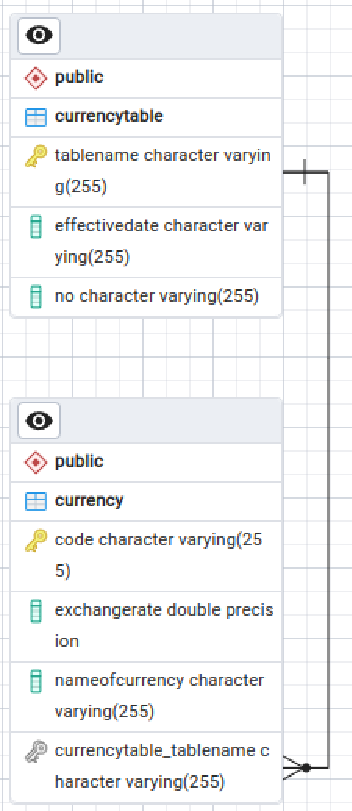
\includegraphics[width=12cm, height=20cm]{ERD.pdf}
\caption{ERD bazy danych}
\label{fig: ERD bazy danych}
\end{figure}

\section{Keycloak}
\label{sec:Keycloak}

Jest to narzędzie open-source służące do uwierzytelniania użytkowników i dostępem do zasobów. Ułatwia czynności związane z bezpieceństwem użytkowników. Nie trzeba zajmować się przechowywaniem danych użytkowników. 

Po zalogowaniu do KeyCloaka nie trzeba powtarzać tej czynności, co oznacza, że nie trzeba korzystać z wielu aplikacji, bo wszystko dostępne jest w jednym miejscu.

KeyCloak umożliwia logowanie przy użyciu sociali takich jak facebook, Github czy Google. Wystarczy dodać taką opcję w konsoli admina. Nie ma potrzeby pisania kodu.

Kolejną możliwościa jest możliwość przechowywania danych w zewnętrznej bazie danych, połaczenie z serwerami \textbf{LDAP} i połączenie z \textbf{Active Directory}.

Keycloak posiada konsole admina, gdzie można przejrzeć wszystkie dostępne możliwości tego narzędzia.

Keylocak posiada również wsparcie dla standardowych protokołów komunikacyjnych, takich jak: OpenID Connect, OAuth 2.0, SAML. 

W stworzonej aplikacji łączę się z \textbf{Keycloackiem} za pomocą następujących zapytań \textbf{HTTP}.

\begin{lstlisting}[breaklines=true]
@RegisterRestClient(baseUri = "http://localhost:8180/")
public interface KeyCloakService {

    @POST
    @Consumes(MediaType.APPLICATION_FORM_URLENCODED)
    @Path("realms/master/protocol/openid-connect/token")
    Response getToken(MultivaluedMap<String, String> formData);

    @POST
    @Consumes(MediaType.APPLICATION_JSON)
    @Path("admin/realms/master/users")
    String register(@HeaderParam("Authorization") String authorizationHeader, String json);
}
\end{lstlisting}

Pierwsze polecenie w powyższym kodzie pobiera \textbf{token} przy prawidłowym zalogowaniu. Ten \textbf{token} później jest potrzebny, aby wykonać akcje dostępne tylko dla zalogowanych użytkowników i posiadających odpowiednią rolę w systemie. W celu zalogowania trzeba wysłać polecenie \textbf{POST} na dany adres, który składa się z nazwy \textbf{localhost} oraz portu, czyli \textbf{http://localhost:8180/} oraz kolejnych wartości, które są specificzne dla tego narzędzia i są one ustawione domyślnie, czyli \textbf{realms/master/protocol/openid-connect/token}. Funkcja przyjmuje jeden argument, którymi są dane logowania opisane w sekcji \ref{sec:endpointy} przy \textbf{endpointcie} logowania.

Drugie polecenie służy do stworzenia użytkownika. Podobnie jak poprzednio część podstawowa adresu jest taka sama, ale pozostałem argumentu się zmienają na \textbf{admin/realms/master/users} i kolejny raz wysyłamy zapytanie typu \textbf{POST}. Tutaj mamy dwa argumentu, gdzie pierwszym jest token logowania użytkownika z rolą admina, żeby mógł utworzyć użytkownika. W kodzie programu są zapisane te dane, więc użytkownik nie musi ich podawać. Drugim elementem są dane do stworzenia nowego użytkownika. Sposób na wykonanie zapytania znajduje się w sekcji \ref{sec:endpointy} przy \textbf{endpointcie} rejestracji.

%%%%%%%%%%%%%%%%%%%%%%%%%%%%%%%%%%%%%%%%%%%%%%%%%%%%%%%%%%%%%%%%
\cleardoublepage
\chapter{Orkiestracja}
\label{cha:Orkiestratory}

Kontenery dostarczają możliwość tworzenia oprogramowania dla
rozwiązań chmurowych i centrów danych. Dzięki nim aplikacja
w każdym systemie zachowuje się tak samo, umożliwiając szybkie
i efektywne ich wzdrażanie. Przy czym, w trakcie rozwoju aplikacji
i jej stopniowemu zwiększaniu się przychodzi potrzeba kontroli
nad cyklem życia projektu i automatyzacji pewnych procesów. 
Pozwalają także uzyskać stałe i nieprzerwane działanie kontenerów, 
monitorowanie stanu systemu, oraz umożliwiają tego samo 
regenerowanie się. Takimi narzędziami są właśnie orkiestratory.\newline


Ważnymi pojęciami odnośnie orkiestracji są: 

\textbf{Continuous Integration (CI)} odnosi się 
do integrowania, budowania i testowania kodu 
w środowisku developerskim. Programiści muszą często 
integrować kod w zdalnych repozytoriach (np. \textbf{Github}).
Od wielkości projektu zależy jak często to ma następować.
Jednak samo dzielenie kodu nie wystarczy, należy go też
sprawdzić, wykonać testy. Wykonywane jest to przez 
\textbf{pipeline}, które dają odpowiednie sygnały czy 
wystąpiły jakieś błędy czy wszystko przebiegło pomyślnie.
\textbf{Continous Integration} powinno być uruchamiane po 
każdym \textbf{commitcie} albo \textbf{pushu}. 

Kolejnym krokiem jest \textbf{Continuous Delivery (CD)}. 
Jest to mechanizm, który występuje wtedy, kiedy ktoś zaaplauduje
zmiane na zdalnym repozytorium i przejdzie pozytywnie testy. 
Wtedy użytkownik może kliknąć przycisk i nowy kod zostanie 
automatycznie zaimportowany na środowisko produkcyjne. 

Jest jeszcze \textbf{Contunuous Deployment (CDP)}, przy którym
nie potrzeba osoby, która potwierdzi wdrożenie. Cały proces 
od \textbf{commita} do wdrożenia na produkcję odbywa się
automatycznie.

W \textbf{Docker Swarmie} można stworzyć wielu klastrów,
gdzie jeden może służyc jako środowisko testowe, a reszta
jako środowisko produkcyjne. W przedstawionym dalej przypadku 
zostanie stworzony tylko jeden klaster w celach testowych. 
Więcej o tym jak podzielić klastry i ustawić w nich środowiska 
testowe i produkcyjne można przeczytać w rozdziale 5 z książki
na pozycji \cite{DockerSwarm}.


W tym rozdziale zostały przedstawione najpopularniejsze 
z nich oraz w jaki sposób zostały skonfigurowane do 
testów opisanych w rozdziale \ref{cha:Opis eksperymentów}.

Jeszcze przed rozpoczęciem konfiguracji, został stworzony 
kontener dla \textbf{Keycloaka}, działa niezależnie do każdego
przedstawionego orkiestratora w tym rozdziale. Jest budowany 
jako zwykły kontener na \textbf{Dockerze} za pomocą komendy:


\begin{lstlisting}[breaklines=true]

docker service create --name pgadmin -p 5050:80 
--network="NBP-APP" -e PGADMIN_DEFAULT_EMAIL="admin@admin.com" 
-e PGADMIN_DEFAULT_PASSWORD="admin" dpage/pgadmin4 

\end{lstlisting}

\section{Docker Swarm}
\label{sec:Docker Swarm}

Przydatne komendy:

\begin{itemize}
\item ,,\textbf{docker swarm init}'' - inicjalizacja Docker Swarm w klastrze, 
\item ,,\textbf{docker service}'' - służy do kontroli serwisu(kontenera) w klastrze. Dostępne parametry to:
\textit{create} do stworzenia serwisu, \textit{ls} do zobaczenia wszystkich serwisów,
\textit{inspect} do sprawdzenia szczegółowych informacji o serwisie,
\textit{scale} do zwiększenia liczby replik serwisu
\item ,,\textbf{docker stack}'' - służy do stworznia lub usunięcia jednego lub wielu serwisów 
zdefiniowanych z pliku \textit{yaml},
\item ,,\textbf{docker network create}'' - służy do utworzenia sieci, która służy 
do komunikacji między serwisami. W Docker Swarmie dodatkowo 
należy dodać wartość \textbf{--driver overlay}.
\end{itemize}


\textbf{Utworzenie smarma:}

Na początku należy utworzyć klaster \textbf{Docker Swarma} przy użyciu \textbf{Advertise address}, którym
jest adres \textbf{IP}. To \textbf{IP} jest potrzebne kiedy klient będzie chciał dołączyć do serwara, więc powinno
się wybrać taki adres, aby każdy mógł się z nim połączyć. W systemie \textbf{Ubuntu} zostało użyte polecenie 
\textbf{ifconfig} i pobrany adres sieci.

\begin{lstlisting}[breaklines=true]
docker swarm init --advertise-address <ip_addr>
\end{lstlisting}

\textbf{Przykładowa odpowiedź:}

\begin{lstlisting}[breaklines=true]
Swarm initialized: current node (jbdzcfqf1er2t96u7z11743xk) is now a manager.

To add a worker to this swarm, run the following command:

    docker swarm join --token SWMTKN-1-6diawyi338mqi75ma5vupxhtezugl3t6xwpiijn2a5uj957922-3k6gfgxj98qjq0mpnelnbpnj2 192.168.65.9:2377

To add a manager to this swarm, run 'docker swarm join-token manager' and follow the instructions.
\end{lstlisting}

Można także przejrzeć listę użytkowników połączonych z danym \textbf{Nodem}
za pomocą komendy \textbf{docker node ls} i wtedy odpowiedź może wyglądać 
w następujący sposób:

\begin{lstlisting}[breaklines=true]
ID                            HOSTNAME         STATUS    AVAILABILITY   MANAGER STATUS   ENGINE VERSION
feszonqwmnbapcv9a76wxq122 *   docker-desktop   Ready     Active         Leader           25.0.3  
\end{lstlisting}

Utworzenie networku z opcją \textbf{overlay}. Pozwala ona 
na komunikację kontenerów utworzonych na różnych klastrach
orkiestratora.Jeśli nie utworzymy sieci to utworzone serwisy połączą się z \textbf{ingressem}. 
Rekomendowane jest utworzenie własnej sieci dla każdej grupy aplikacji,
które mają pracować razem. 

\begin{lstlisting}[breaklines=true]
docker network create --driver overlay NBP-APP
\end{lstlisting}

\textbf{Najpierw należy stworzyć serwis bazy danych:}

\begin{lstlisting}[breaklines=true]
version: '3.8'

services:
  postgresql:
    image: postgres
    deploy:
      replicas: 1
      placement:
        constraints:
          - node.role == manager
      restart_policy:
        condition: any
    ports:
      - "5432:5432"
    networks:
      - NBP-APP
    environment:
      - POSTGRES_PASSWORD=admin
      - PGDATA=/var/lib/postgresql/data/pgdata
    volumes:
      - pg_data:/var/lib/postgresql/data/pgdata

networks:
  NBP-APP:
    external: true

volumes:
  pg_data:
    driver: local
\end{lstlisting}

W powyższym kodzie został ustawiony obraz bazodanowy postgres, 
liczba replik na 1, port na 5432. W \textbf{environment} zostało 
ustawione hasło oraz miejsce magazynowania danych bazodanowych. 
Połączone również zostało z wcześniej utworzoną siecią NBP-APP, 
co spowodowało, że połączenie z bazą danych wenątrz danej sieci
będzie można uzyskać ustawiając adres na \textbf{host.docker.internal}.

\begin{lstlisting}[breaklines=true]
quarkus.datasource.jdbc.url=jdbc:postgresql://host.docker.internal:5432/postgres
quarkus.datasource.password = admin
quarkus.datasource.username = postgres
\end{lstlisting}

\textbf{Następnie tworzona jest aplikacja za pomocą 
następującego kodu:}

\begin{lstlisting}[breaklines=true]
version: '3.8'

services:
  nbp-app:
    image: matiuw/nbp-app:latest
    deploy:
      replicas: 1
      placement:
        constraints:
          - node.role == manager
      restart_policy:
        condition: any
    ports:
      - "8080:8080"
    networks:
      - NBP-APP

networks:
  NBP-APP:
    external: true
\end{lstlisting}

W powyższym przykładzie został stworzony serwis 
wykorzystujący utworzony obraz aplikacji przesłanej
na zdalne repozytorium \textbf{Docker Hub}. Aplikacja jest
dostępna na porcie 8080 i dołączona do sieci NBP-APP.

Utworzona architektura jest dostępna na obrazku \ref{fig: Architektura aplikacji w Docker Swarmie}.

\begin{figure}[!h]
  \centering
  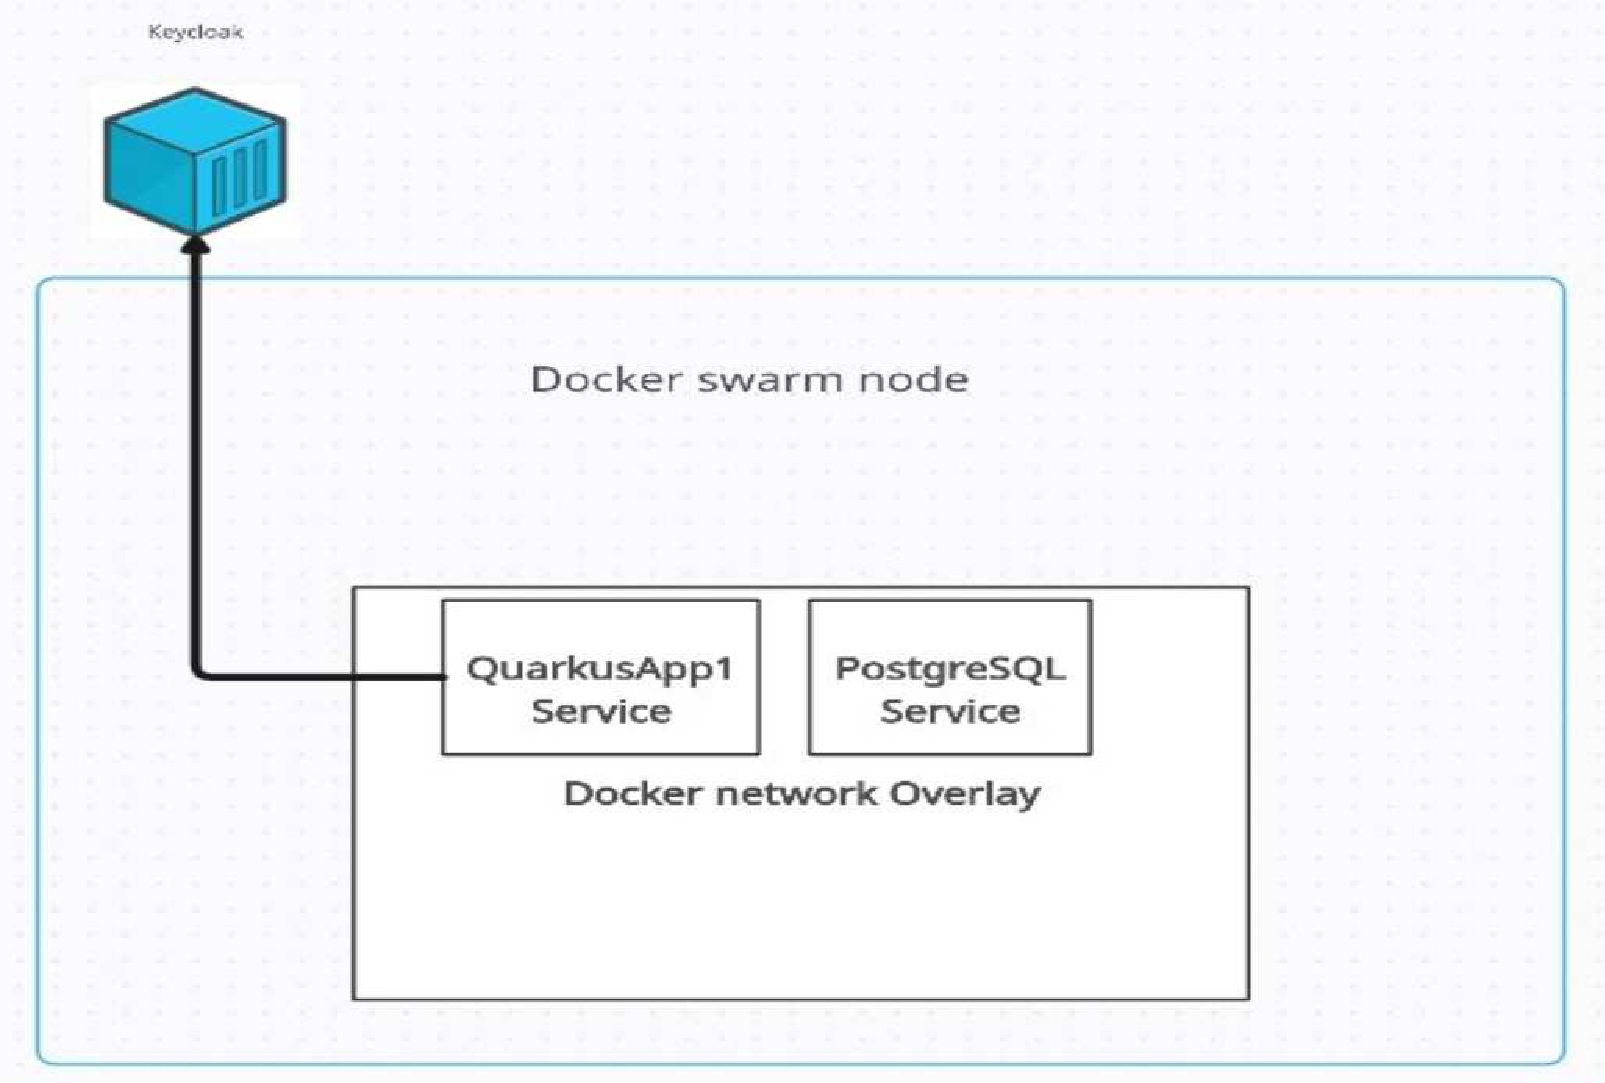
\includegraphics[width=12cm]{swarm/AplikacjaDockerSwarm.pdf}
  \caption{Architektura aplikacji w Docker Swarmie}
  \label{fig: Architektura aplikacji w Docker Swarmie}
\end{figure}

Sczegółowy sposób uruchomienia został opisany w rozdziale 3 
w pozycji \cite{DockerSwarm}.

\section{Kubernetes}
\label{sec: Kubernetes}

Architektura Kubernetesa składa się z przynajmniej 
jednego \textbf{master node} połączonego z \textbf{worker
nodes}. Każdy z \textbf{worker nodów} posiada proces 
o nazwie \textbf{cubelet}, który pozwala innym \textbf{nodom}
komunikować się między sobą oraz przeprowadzać zadania na nich.
Na przykład uruchamiać aplikacje. Na każdym \textbf{worker
nodzie} uruchomione są aplikacje zamknięte w koneterach. 
Na \textbf{master nodzie} uruchomione procesy, które są
niezbędne do prawidłowego działania klastra. Jednym z takich
procesów jest \textbf{Api Server}, który jest punktem wejścia
dla \textbf{klastra Kubernetesa}. Jest to proces do którego 
będą się komunikować takie elementy jak \textbf{kubernetes 
dashboard} i narzędzie linii poleceń. Kolejnym procesem jest
\textbf{Controller manager}, którego zadaniem jest kontrola 
nad tym co się dzieje wewnątrz klastra. Jego zadaniem jest
na przykład odbudowa \textbf{poda}, gdy wystąpi jakiś błąd lub
jego restart. Trzecim procesem jest \textbf{Scheduler}, którego
zadaniem jest obserwowanie API serwera w poszukiwaniu nowego
zadania i przydzielenie odpowiedniego \textbf{worker noda}.
Czwartym procesem jest \textbf{etcd}, który przetrzymuje stan
\textbf{klastra Kubernetesa}. Zatem posiada wszystkie dane 
odnośnie każdego noda i każdego kontenera. Dane zapisane w tym
procesie wykorzystywane są w przypadku zrobienia 
\textbf{Backupu}. Komponent umożliwiający \textbf{worker i master 
nodom} porozumiewanie się między sobą jest \textbf{virtual network}.

Do uruchomienie Kubernetesa lokalnie na komputerze został 
wykorzystany \textbf{Minikube}. Zostało stworzone przez
Google w 2016 i obecnie jest jednym z popularniejszych 
sposob na uruchomienie klastra \textbf{Kubernetesa} 
lokalnie. Uruchomieie jest proste, gdyż wymaga jedynie 
użycia komendy \textbf{minikube start} i cała konfiguracja
wykona się automatycznie. Zostanie wybrany odpowiedni 
\textbf{driver (domyślnie Docker)} oraz przypisane 
odpowiednie zasoby komputera. 

Dodatkowo jest możliwość włączenia graficznego interfeju
za pomocą komendy \textbf{minikube dashboard}. Pozwala on 
wdrażać skonteneryzowane aplikacje do klastra 
\textbf{Kubernetesa}. Rozwiązywać problemy odnośnie 
aplikacji. Zarządzać zasobami klastra. Pobierać informacje 
o podach i aplikacjach uruchomionych w klastrze. Tworzyć 
i modyfikować indywidualne elementy \textbf{Kubernetesa}.

Do \textbf{Minikube} dołączona też jest aplikacja
służąca do komunikacji między API Kubernetesa, a systemem 
sterowania za pomocą linii poleceń. Zaczyna się polecenia
od nazwy \textbf{kubectl}. Pozwala wykonać operacje 
za pomocą komend. Poniżej kilka z nich, które sa 
wykorzystywane do wzdrożenia aplikacji:

\begin{itemize}
  \item Node - jest to fizyczna lub wirtualna maszyna

  \item Pod - najmniejsza jednostka w \textbf{Kubernetesie},
  jest to abstrakcja nad kontenerem. Jego zadaniem jest
  uruchomienie środowiska albo powłoki nad kontenerem. 
  Zazwyczaj w jednym \textbf{podzie} jest jeden kontener.
  W specyficzny przypadkach można uruchomić więcej kontenerów
  w ramach \textbf{poda}, lecz nie jest to zalecane. Każdy 
  \textbf{pod} posiada swój własny adres IP i możliwa jest
  komunikacją między \textbf{podami} za pomocą tego adresu.
  
  \item Service - jest to statyczny lub penamentny adres IP,
  który może być dołączony do poda. Jednocześnie pod i service
  działają niezależnie, więc jeśli coś się stanie z podem to
  service wciąż będzie działał.
  
  \item Ingress - zamiast łączenia się przy pomocy adresu IP,
  można wykorzstać ten element w celu nadania nazwy dla servicu.
  Przykładowo zamiast łączyć sie z adresem http://192.168.0.1:8080
  można ustawić to na https://nbp-app:8080 z nazwą domeny 
  i szyfrowanym połączeniem. Zapytania w ten sposób będą 
  najpierw trafiać do ingressa i następnie do servicu. 

  \item ConfigMap - jest to zewnętrzna konfiguracja dla aplikacji.
   Przydaje się w sytuacji, gdyby zaszła potrzeba zmiany nazwy 
   aplikacji to wtedy trzeba zmienić to w aplikacji, zbudować 
   ją, wysłać na repozytorium i z powrotem zbudować poda. 
   Za pomocą configmapy możemy pominąć wszystkie te kroki. 
   Configmap również może przetrzymywać dane logowania do bazy 
   danych, lecz dane te są dostępne i nie są zakodowane.

  \item Secret - działa podobnie do configmapy, ale służy do 
  przechowywania danych wrażliwych. Dane wenątrz są zakodowane 
  za pomocą algorytmu base 64. Dane te nie są całkowicie 
  zabezpieczone, ponieważ każdy kto posiada dostęp do API może
  zobaczyć te dane i je zmodyfikować. Również osoby, które mają
  zezwolenia do tworzenia podów mają dostęp do secretu. 
  Aby w pełni zabezpieczyć takie dane należy zainstalować aplikacje
  zewnętrzne. Innym zastosowaniem secretów może być trzymanie 
  wewnątrz nich zmiennych środowiskowych i parametrów aplikacji.

  \item Volume - służy do przechowywania danych na przykład
  z bazy danych na fizycznym nośniku. Przydaje się w przypadku 
  wystąpienia awarii dla poda posiadajacego bazę danych lub coś
  innego posiadającego swój stan. Miejscem przechowywania może 
  być lokalnie dysk ssd na komputerze lub zdalnie, poza
  klastrem Kubernetesa.  

  \item Deployment - w czasie tworzenia i działania aplikacji
  występują błędy powodujące przerwanie działania aplikacji.
  Kubernetes oferuje mechanizm auto regeneracji poda, lecz 
  czasie w którym to następuje użytkownik, nie ma dostępu do 
  aplikacji. Z pomocą przychodzi deplyoment, który tworzy
  repliki podów i natychmiast zastępuje niedziałającego poda
  na takiego wolnego od błędów. Pozwala on na ustalenie liczby
  replik podów. Jest to kolejna warstwa abstrakcji nad podami.
  Co za tym idzie powinno się pracować nad deploymentem, a nie
  nad podami. Nie można zastosować deplyomentu w przypadku 
  baz danych, ponieważ mają swój stan, czyli dane. Trzeba ustalić,
  który pod ma obecnie uprawnienia do dostępu do tych danych.
  Potrzebny jest mechanizm pozwalający zarządzać dostępem do miejsca 
  przechowywania danych w celu uniknięcia niespójności danych.
  
  \item StatefulSet - używane jest do aplikacji jak bazy danych: 
  MySQL, Elastic Search, mongoDB i innych aplikacji posiadających
  swój stan. Podobnie jak deployment jego zadaniem jest 
  replikacja podów oraz ich skalowanie, ale również zapewnia
  synchroniczność dostępu do bazy danych.

\end{itemize}

Informacje o elementach Kubernetesa można znaleźć przykładowo 
w książce na pozycji \cite{Kubernetes}.
  
\subsection{Uruchomienie aplikacji}

Do stworzenia każdego elementu Kubernetesa zostały wykorzystane
pliki konfiguracyjne, które składają się z następujących 3 części.
Początek każdego pliku zawiera informacje o wersji i odpowiedzi,
jakiego elementu kubernetesa dotyczy: poda, servicu itp. Pierwsza
część zawiera informacje o metadatach, druga część informuje
o specyfikacji, czyli przykładowo o nazwie i obrazie. Ostatnia
część mówi o statusie, którego dane pobierane są z etcd.

Stworzenie bazy danych za pomocą komendy
\textbf{kubectl apply -f postgresPod.yml.}

\begin{lstlisting}[breaklines=true]
apiVersion: v1
kind: Pod
metadata:
  name: pg-pod
  labels:
    name: postgres
spec:
  containers:
  - name: postgres
    image: postgres:12.3
    imagePullPolicy: IfNotPresent
    ports:
    - name: pg-port
      containerPort: 5432
    env:
    - name: POSTGRES_PASSWORD
      value: admin
    - name: PGDATA
      value: /data/k8s
    volumeMounts:
    - name: pg-vol
      mountPath: /data
    securityContext:
      runAsUser: 0
      runAsGroup: 0
  volumes:
  - name: pg-vol
    hostPath:
      path: /data
      # path: /Users/<>/minikube/pgdata
  restartPolicy: Never
  securityContext:
    runAsUser: 1000
    runAsGroup: 1000
    fsGroup: 1000

\end{lstlisting}

Kolejnym krokiem jest stworzenie Deploymentu
dla aplikacji za pomocą komendy \textbf{kubectl apply -f 
quarkusDeployment.yml }. Komunikacja między 
\textbf{podami} w ramach tego samego klastra
odbywa się wykorzystując ich adresy \textbf{IP}. Można
to zrobić za pomocą komendy \textbf{kubectl describe 
pod nazwa-poda}. I następnie należy zaktualizować
\textbf{application.properties} w aplikacji o nowy adres
dla bazy danych.

plik quarkusDeployment.yml

\begin{lstlisting}[breaklines=true]
apiVersion: apps/v1
kind: Deployment
metadata:
  name: nbp-app
spec:
  replicas: 1
  selector:
    matchLabels:
      app: nbp-app
  template:
    metadata:
      labels:
        app: nbp-app
    spec:
      containers:
      - name: nbp-app
        image: matiuw/nbp-appkubernetes:latest

\end{lstlisting}

Następnie trzeba utworzyć serwis.

\begin{lstlisting}[breaklines=true]
apiVersion: v1
kind: Service
metadata:
  name: nbp-app
spec:
  selector:
    app: nbp-app
  ports:
    - protocol: TCP
      port: 8080
      targetPort: 8080
  type: LoadBalancer

\end{lstlisting}

Ostatnim krokiem jest wystawienie aplikacji na dostęp
zewnętrzny. Można to zrobić na 2 sposoby. Z użyciem 
\textbf{NodePortu} oraz \textbf{LoadBalancera}. W tym
przypadku został wykorzystany drugi sposób, ponieważ
przypisuje on każdemu \textbf{serwisowi} własny adres \textbf{IP}. \textbf{LoadBalancera} używa się poprzez wpisanie na nowej konsoli komendy \textbf{minikube tunnel}. Utworzy się ścieżka między hostem, a serwisem CIDR klastra używając IP klastra jako bramę. Tunnel wystawia zewnętrzne IP bezpośrednio do jakiegokolwiek programu na systemie operacyjnym hosta. \newline

Przykład odpowiedzi dla komendy \textbf{kubectl get svc} przed użyciem \textbf{tunnelu}.

\begin{lstlisting}[breaklines=true]
  nbp-app      LoadBalancer   10.106.154.68   <pending>     8080:32735/TCP   50s

\end{lstlisting}

Oraz po użyciu \textbf{tunnelu}.

\begin{lstlisting}[breaklines=true]
  nbp-app      LoadBalancer   10.106.154.68   127.0.0.1     8080:32735/TCP   10m
\end{lstlisting}

Obraz całości można zobaczyć na obrazku \ref{fig: Architektura aplikacji w Kubernetesie}

\begin{figure}[!h]
\centering
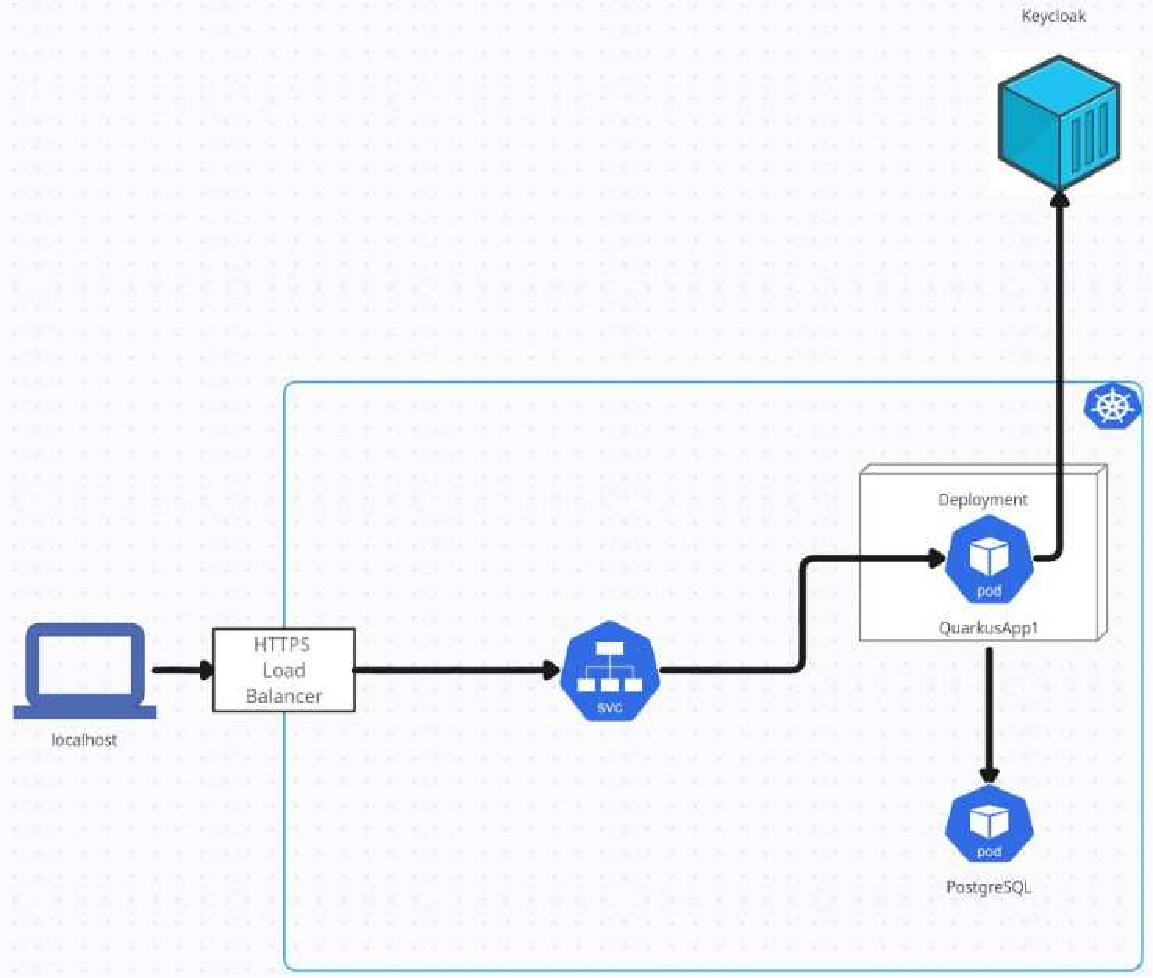
\includegraphics[width=12cm]{kubernetes/AplikacjaKubernetes.pdf}
\caption{Architektura aplikacji w Kubernetesie}
\label{fig: Architektura aplikacji w Kubernetesie}
\end{figure}

\section{Nomad Hashicorp}

Jest to mniej popularny orkiestrator od dwóch poprzednich. Został
stworzony przez fimę HashiCorp. Charakteryzuje się on:

\begin{itemize}
  \item ,,\textbf{Inteligentne zarządzanie zasobami}'' - Nomad
  optymalizuje zasoby przypisane do klastra poprzez efektywne 
  obciążenia między nodami w klastrze używając procesu zwanego 
  \textbf{bin packing}, 
  \item ,,\textbf{Samo regeneracja}'' - stałe spawdzanie 
  i kontrola nad aktywnymi kontenerami i podjęcie 
  odpowiednich działań w przypadku wystąpienia błędów,
  \item ,,\textbf{Ciągłe działanie aplikacji}'' - wsparcie 
  dla wielu strategii aktualizacji oprogramowania, np. 
  textbf{rolling updates, blue/green deployments, canary
  deployments},
  \item ,,\textbf{Różne typy obciążeń}'' - elastyczność Nomada
  pochodzi z \textbf{task driverów} pozwalając na orkiestrację
  Dockera i innych kontenerów, jak i również dla wykonywalnych 
  plików Jar, wirtualnych maszyn QEMU, czystych poleceń \textbf{exec driver},
  oraz daje możliwość dla użytkowników stworzenia ich własnych
  driverów,
  \item ,,\textbf{Wsparcie dla wielu systemów operacyjnych}'' - 
  Nomad uruchamia się jako typ binarny i pozwala orkiestrować
  aplikacje jednocześnie na macOS, Windowsie i Linuxie,
  \item ,,\textbf{Zunifikowany przepływ pracy}'' - bez względu
  na to czy zadaniem jest zarządzanie kontenerami, aplikacjami Java
  maszynami wirtualnymi to w Nomadzie sposób zarządzania nimi
  jest jednakowy,
  \item ,,\textbf{Deklaratywna specyfikacja zadania}'' - użytkownik 
  podaje co chce zrobić, a Nomad zajmuje się resztą.
\end{itemize}


Konfiguracja Nomada składa się z: 
\begin{itemize}
  \item ,,\textbf{agent}'' - jest to proces Nomada działający
  na serwerze albo jako tryb klienta,
  \item ,,\textbf{client}'' - jest odpowiedzialny za uruchomienie, 
  które są do niego przypisane. Sprawdza czy jakieś zadania 
  muszą być przydzielone. Kiedy agent jest uruchomiony, client
  staje się nodem,
  \item ,,\textbf{server}'' - jego zadaniem jest zarządzanie wszystkimi
  jobsami i clientami. Serwer monitoruje stan zadań i sprawdza, 
  czy działają prawidłowo. Decyduje również jakie zadania 
  na jakich węzłach klienckich powinny zostać umieszczone, 
  uwzględniając zasoby i wymagania tych zadań. Między serwerami
  następuje wymiana danych, dzięki czemu jeśli jeden z serwerów
  przestanie działac to inny będzie mógł go zastąpić. Powoduje to, 
  że klaster jest cały czas dostępny,
  \item ,,\textbf{dev agent}'' - jest to tryb, który przydaje 
  się podczas tworzenia i testowania aplikacji, ponieważ można 
  szybko i łatwo uruchamiać aplikacje bez skomplikowanej 
  konfiguracji. Agent działa jednocześnie jako klient i serwer,
  co ułatwia testowanie. Agent nie zapisuje swojego stanu, więc 
  po restarcie dane zostaną utracone. Co również może być zaletą, 
  bo nie trzeba usuwać pozostałości i można wszystko od początku 
  przetestować.
\end{itemize}


Najważniejsze operacje Nomada to:
\begin{itemize}
  \item ,,\textbf{task}'' - jest to podstawowym elementem w Nomadzie. 
  Są wykonywane przez \textbf{taks drivers} takie jak docker albo exec,
  \item ,,\textbf{group}'' - jest to zbiór tasków, które są uruchamiane 
  na tym samym clientcie,
  \item ,,\textbf{job}'' - główna jednostka zarządzania w Nomadzie, 
  za pomocą niej definiuje się i zarządza się aplikacjami. Zawiera wszystkie 
  informacje potrzebne do ich uruchomienia. Job określa w jaki sposób 
  aplikacja ma być uruchamiana. Job składa się z jednego lub więcej tasków,
  \item ,,\textbf{job specification}'' - jest to plik w którym jest określony 
  schemat działania dla jobów. Określa typ dla jobów, zadania i potrzebne 
  zasoby sprzętowe oraz zawiera informacje dotyczące, który client ma uruchomić 
  danego joba,
  \item ,,\textbf{allocation}'' - określa specyfikacje dla jobów. Opisuje typ joba, 
  jego zadania i zasoby potrzebne do uruchomienia.
\end{itemize}

Dokładny opis tych elementów Nomada można znaleźć w dokumentacji technicznej
dostępnej pod adresem \cite{Nomadwww}.


Uruchomienie klastra odbywa się za pomocą komendy: 

\begin{lstlisting}[breaklines=true]
sudo nomad agent -dev -bind 0.0.0.0 -network-interface='{{ GetDefaultInterfaces | attr "name" }}' export NOMAD_ADDR=http://localhost:4646
\end{lstlisting}

Następnie jest uruchamiany \textbf{consul} \ref{sec:Consul} 
za pomocą komendy:

\begin{lstlisting}[breaklines=true]
  consul agent -dev -bind=0.0.0.0 -advertise=<your_advertise_address> -log-level=INFO
\end{lstlisting}

Gdzie \textbf{adverise} jest to adres IP komputera. Po tym
można już zacząć tworzyć bazę danych oraz uruchomić aplikację.
Jako adres po którym będzie można się komunikować z nimi będzie 
adres IP komputera. Najpierw kod uruchamiający postgresa 
za pomocą konedy \textbf{nomad job run -hcl1 
nbpapppostgres.nomad.hcl}: 

\begin{lstlisting}[breaklines=true]

job "postgres" {
  datacenters = ["dc1"]
  type = "service"

  group "postgres" {
    count = 1

    task "postgres" {
      driver = "docker"
      config {
        image = "postgres"
        ports = ["db", "http"]
      }
      env {
          POSTGRES_USER="postgres"
          POSTGRES_PASSWORD="admin"
      }

      logs {
        max_files     = 5
        max_file_size = 15
      }

      resources {
        cpu = 1000
        memory = 1024
      }
      service {
        name = "postgres"
        tags = ["postgres for vault"]
        port = "db"

        check {
          name     = "alive"
          type     = "tcp"
          interval = "10s"
          timeout  = "2s"
        }
      }

    }
    restart {
      attempts = 10
      interval = "5m"
      delay = "25s"
      mode = "delay"
    }
    network {
      mbits = 10
      port  "db"  {
        static = 5432
      }
      port "http" {
        to = 8080
      }
    }
  }
  update {
    max_parallel = 1
    min_healthy_time = "5s"
    healthy_deadline = "5m"
    auto_revert = false
    canary = 0
  }
}

\end{lstlisting}

Następnie kod uruchamiający aplikację 
\textbf{nomad job run -hcl1 nbpAppQuarkus.nomad.hcl}:

\begin{lstlisting}[breaklines=true]

  job "nbpapp" {
    datacenters = ["dc1"]
    type        = "service"
  
    group "web" {
      count = 1
  
      network {
        port "quarkus"
        {
          to = 8080
        }
      }
  
      task "service" {
        driver = "docker"
  
        config {
          image        = "matiuw/nbp-appnomad:latest"
          network_mode = "host"
          ports        = ["quarkus"]
        }
      }
    }
  }
  
\end{lstlisting}

\begin{figure}[!h]
\centering
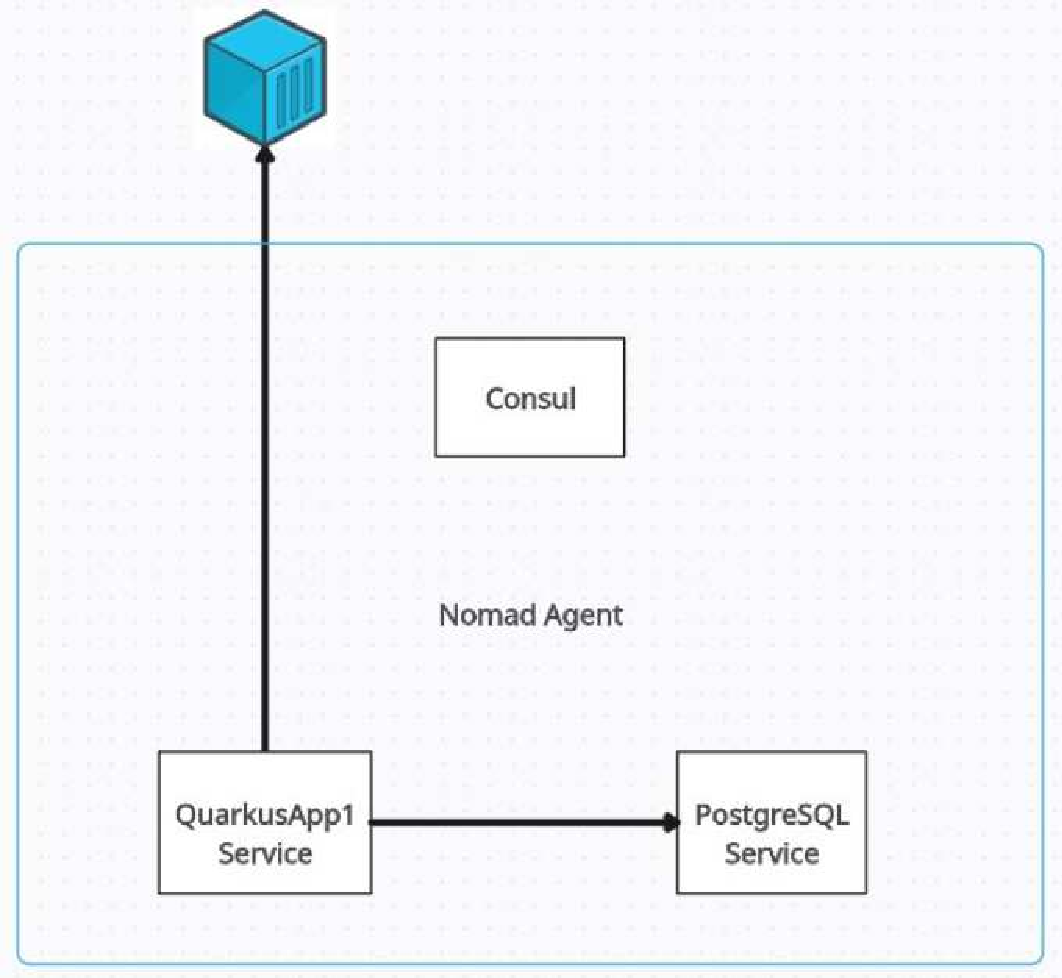
\includegraphics[width=12cm]{nomad/AplikacjaNomad.pdf}
\caption{Architektura aplikacji w Nomadzie}
\label{fig: Architektura aplikacji w Nomadzie}
\end{figure}

Jest to narzędzie stworzone przez firmę HasiCorp. Link do dokumentacji
dostępny jest na pozycji \cite{Consulwww}. Jest to serwis 

%%%%%%%%%%%%%%%%%%%%%%%%%%%%%%%%%%%%%%%%%%%%%%%%%%%%%%%%%%%%%%%%
\cleardoublepage
\chapter{Opis przeprowadzonych eksperymentów}
\label{cha:Opis eksperymentów}

W tym rozdziale został przedstawiony opis przeprowadzonych eksperymentów. Jakie narzędzia zostały użyte oraz opis przeprowadzonych czynności. 

\section{Platforma testowa}

Stanowiskiem do testowania jest komputer stacjonarny o następujących parametrach.

\begin{itemize}
    \item ,,\textbf{Procesor}'' - AMD Ryzen 5 5600X, 
    \item ,,\textbf{Pamięć ram}'' -  Crucial 32GB (2x16GB) 3600MHz CL16 Ballistix Black,
    \item ,,\textbf{Dysk SSD}'' -  GOODRAM 256GB 2,5" SATA SSD CX400,
    \item ,,\textbf{System operacyjny}'' - Ubuntu 22.04.4 LTS,
\end{itemize}

W przypadku innych konfiguracji wyniki będą się różniły.

\section{Eksperyment obciążenia procesora i użycia pamięci}

W tym eksperymencie zostały przeprowadzone testy użycia 
najważniejszych parametrów w komputerze, czyli pamięci 
operacyjnej oraz procesora.Dane w przypadku Docker Swarma zostały 
pozyskane przy pomocy narzędzia Swarmprom. W przypadku 
\textbf{Kubernetesa} został użyty addon, który można zainstalować 
za pomocą komendy \textbf{minikube addons enable metrics-server}, 
a w przypadku \textbf{Nomada} nie trzeba było nic dodatkowo instalować.

Przyjęta jednostką użycia pamięci zostały MB. W 
\textbf{Kubernetes} i \textbf{Nomadzie} nie przedstawiały wyników 
w tej jednostce, więc zaszła potrzeba dopasowania tego. Tą jednostką 
są MiB, czyli mebibity. Jest to jednostka binarna. Przykładowo 1MiB 
posiada mnożnik $2^20 = 1024^2$, gdzie 1MB ma mnożnik $10^6$. 
Zatem powinno się przeliczyć to za pomocą następującego wzoru: 
$1 MiB = 1024^2 B = 1048576 B = 1.048576 MB$. 

W przypadku użycia procesora trudno porównać uzyskane wyniki z powodu 
różnych jednostek pomiarowych. \textbf{Swarmprom} użycie procesora 
przedstawia w procentach. Kubernetes z drugiej strony przedstawia 
wyniki w wirtualnych CPU, gdzie jedna jednostka CPU oznacza jeden 
rdzeń CPU. Jeśli się nie sprecyzuje ilość przeznaczonych zasobów to 
dla jednego \textbf{poda} przypisane jest 1m co jest równe 0.001 CPU.

Dane w \textbf{Nomadzie} są podawane w Mhz co znacząco utrudnia 
porównanie wyników. Żeby zamienić wyniki z procent na Mhz trzeba 
pobrać wyniki aktualnego użycia rdzenia, co jest trudne do wykonania.

\subsection{Swarmprom}

Jest to zbiór narzędzi do monitorowania użytych zasobów przez serwisy w \textbf{Docker Swarmie}. W jego skład wchodzą:

\begin{itemize}
    \item ,,\textbf{Prometheus}'' - narzędzie \textbf{open source} służące do monitorowania, gromadzenia i powiadamiania o danych z klastra \textbf{Docker Swarm}, 
    \item ,,\textbf{Grafana}'' - służy do prezentowania danych otrzymany z \textbf{Prometheusa} i na ich podstawie tworzenie wykresów i tabel, 
    \item ,,\textbf{cAdvisor}'' - jest to narzędzie \textbf{pen source} stworzone przez \textbf{Google} do monitorowania kontenerów. Zbiera, zegreguje i eksportuje dane odnośnie kontenerów takie jak CPU i użycie pamięci, system plików i statystyki sieci, 
    \item ,,\textbf{alertmanager}'' - służy do odbierania i przetwarzania alertów z takich narzędzi jak \textbf{Prometheus}. Odpowiednio przetwarza te dane usuwając duplikaty, grupuje dane i przekazuje bezpośrednio do miejsca docelowego, 
    \item ,,\textbf{unsee}'' - narzędzie do wizualizacji i zarządzania alertami w systemach monitorowania, 
    \item ,,\textbf{node-exporter}'' - służy do zbierania metryk systemu i przekazywania ich z formacie w ktorym może być zrozumiały dla \textbf{Prometheusa}.
\end{itemize}

Indywidualne isntalacje poszczególnych elementów
zostały opisane w rozdziale 10 w ksiażce 
na pozycji \cite{DockerSwarm}.

\section{Eksperyment startu aplikacji}

Czas budowania jest istotnym elementem porównawczym między orkiestratorami. Podczas pracy wiele razy tworzy się i usuwa serwisy. 

Celem testu jest sprawdzenie czasu jaki potrzebuje dany orkiestrator od momentu rozpoczęcia budowania aplikacji, aż do uzyskania prawidłowej odpowiedzi z zapytania HTTP. Kod testujący czas startu serwisu w Docker Swarmie: 

\begin{lstlisting}[breaklines=true]

#include <stdio.h>
#include <stdlib.h>
#include <string.h>
#include <unistd.h>
#include <stdint.h>
#include <sys/time.h>
#define BUFFER\_SIZE 128\newline

int containsExchangeValue(const char *buffer) \{
    return strstr(buffer, "3.95") != NULL; 
}

long long timeInMilliseconds(void) \{
    struct timeval tv;

    gettimeofday(&tv,NULL);
    return (((long long)tv.tv_sec)*1000)+(tv.tv_usec/1000);
}

void writeToFile(double execution_time) {
    FILE *file = fopen("wyniki.txt", "a");
    if (file == NULL) {
        printf("Błąd podczas otwierania pliku.\n");
        return;
    }

    fprintf(file, "%.4f\n", execution_time);
    fclose(file);
}

void startProgram(char *buffer, FILE *curl_output) {

    long long start_time, end_time;
    double execution_time;

    start_time = timeInMilliseconds();

    FILE *fp = popen("docker service create --name NBP-APP -p 8080:8080 --network=NBP-APP matiuw/nbp-app:latest", "r");
    pclose(fp);

    do {
        curl_output = popen("curl -X GET -H \"Content-Type: application/json\" -d '{\"amount\": 1, \"myCurrency\": \"USD\", \"targetCurrency\": \"PLN\"}' http://localhost:8080/currency/currencyExchangeValue", "r");
        
        fgets(buffer, BUFFER_SIZE, curl_output);

    } while(!containsExchangeValue(buffer));

    pclose(curl_output);

    memset(buffer, 0, sizeof(buffer1));

    end_time = timeInMilliseconds();
    execution_time = (double)(end_time - start_time) / 1000; 
    printf("Czas wykonania: %.4f sekund.\n", execution_time);

    writeToFile(execution_time);

    fp = popen("docker service rm NBP-APP", "r");
    pclose(fp);
}

int main() {

    char buffer[BUFFER_SIZE];
    FILE *curl_output;

    for(int i = 0; i < 1; i++) {
        startProgram(buffer, curl_output);
        sleep(15);
    }

    return 0;
}

\end{lstlisting}

Powyższy kod składa się z następujących kroków. W funkcji \textbf{main} jest tworzony \textbf{buffer} oraz pętla, która odpowiada za ilość przeprowadzonych testów. Między testami jest przerwa wykonana za pomocą funkcji \textbf{sleep(x)}. Na początku funkcji \textbf{startProgram()} następuje pobranie czasu początkowego oraz wykonanie komendy utworzenia serwisu w \textbf{Docker Swarmie} (w przypadku Kubernetesa jest tworzony deployment, a w przypadku Nomada jest tworzony nowy \textbf{job}). W pętli do while wykonywane jest polecenia GET i wynik zapisywany jest do buffora za pomocą funkcji fgets. Pętla się kończy w przypadku pobrania prawidłowej odpowiedzi, która jest sprawdzana w funkcji \textbf{containsExchangeValue()}. Po zakończeniu pętli czyszczony jest \textbf{buffor} oraz ponownie pobierany jest czas zakończenia działania. Za pomocą tych dwóch czasów obliczana jest różnica, która jest wynikiem działania programu i jest on zapisywany do pliku. Na koniec usuwany jest serwis, żeby móc wszystkie kroki powtórzyć od początku. Średni czas uruchomienia na podstawie 100 takich uruchomień można znaleźć w sekcji \ref{sec:StartAplikacji}.

\section{Eksperyment stabilności działania}

Eksperyment stabilności działania został przeprowadzony przy użyciu narzędzia \textbf{Gatling}. Służy do sprawdzenia czy w aplikacji pojawią się błędy w przypadku dużej liczby użytkowników próbujących się połączyć w tym samym czasie. Dzięki, temu część błędów można jeszcze wykryć przed wypuszczeniem kodu na produkcję.

Jest to narzędzie napisane w \textbf{Scali} 2.12.10 i potrzebuje do działania również \textbf{Javę 1.8}, gdyż jest to język, który korzysta z maszyny wirtualnej \textbf{Javy} jako platformy uruchomieniowej.

Utworzony kod programu: 

\begin{lstlisting}[breaklines=true]

class MySimulation extends Simulation {

  //protocol
  val httpProtocol = http
    .baseUrl("http://localhost:8080")

  //scenario
  val scn1 = scenario("Przelicz kurs").exec(
    http("Przelicz kurs req")
      .get("/currency/getCurrency/table/A/value/1")
      .header("content-type", "application/json")
      .asJson
//      .body(StringBody(
//        """
//          |{
//          |      "amount": 1,
//          |      "myCurrency": "USD",
//          |      "targetCurrency": "PLN"
//          |}
//          |""".stripMargin)).asJson
      .check(
        status is 200,
        jsonPath("$.code") is "BGN"
      )
  )

  //setup
  setUp(scn1.inject(rampUsers(6000).during(30))
  ).protocols(httpProtocol)

}

\end{lstlisting}

W powyższym kodzie została utworzona klasa rozszerzająca klasę \textbf{Simulation}. Kod programu składa się z 3 częsci. Pierwsza z nich określa główną część adresu \textbf{http}. W drugiej zdefiniowana jest metoda \textbf{http} oraz argumenty \textbf{linku}, ciało metody oraz przewidywany rezultat polecenia. W ostatniej zostały zdefiniowane informacje na temat tego ile ma się wykonać zapytań i w jakim czasie. 
\newline

Po wynanym teście generowany jest raport w postaci \textbf{strony www}.  

%%%%%%%%%%%%%%%%%%%%%%%%%%%%%%%%%%%%%%%%%%%%%%%%%%%%%%%%%%%%%%%%
\cleardoublepage
\chapter{Analiza}
\label{cha:Analiza Wynikow}

\section{Wyniki i wnioski obciążenia procesora i użycia pamięci}
\label{sec:Zarzadzanie zasobami}

Wyniki dla użycia procesora zostały przedstawione na rysunku 
\ref{fig: Uzycie procesora}. Jednostką wspólną zostały MHz. 
W przypadku Kubernetesa i Nomada wyniki 5 instancji są 
wielokrotnościa wyniku dla 1 instancji, a w przypadku Docker 
Swarma dla jednej instacji wynik wyszedł 3,22 MHz, a dla 
5 instancji 13,8 MHz. Wyniki zostały pobrane, gdy orkiestratory 
były bez obciążenia.

\begin{figure}[!h]
  \centering
  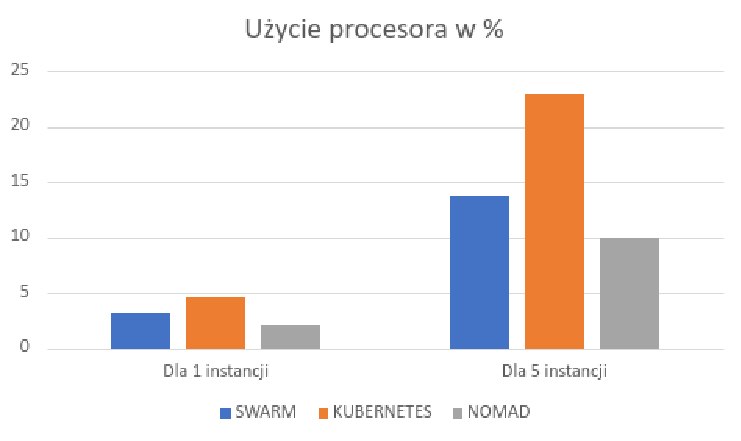
\includegraphics[width=12cm]{uzycieProcesora.pdf}
  \caption{Wyniki użycia procesora dla aplikacji w orkiestratorach}
  \label{fig: Uzycie procesora}
\end{figure}

Porównanie użycia pamięci i obciążenia procesora między orkiestratorami
jest trudne, ponieważ wszystkie mają mechanizmy zarządzania zasobami. W ten
sposób ilość przydzielonych zasobów może się różnić w czasie. Przy uruchomieniu 
aplikacji orkiestrator przydziela pewną ilość tych zasobów i po wykonaniu 
zapytania do aplikacji ta ilość może się zwiększyć dynamicznie.

Kontrola nad tym jest bardzo ważna. W systemach na Linuxie, jeśli jądro systemu
wykryje, że nie ma wystarczająco pamięci, aby uruchomić ważne funkcje systemu, to
wyrzuci błąd \textbf{Out of Memory Exception} i zacznie zabijać mniej ważne procesy, 
aby zwolnić tą pamięć. Również aplikacje uruchomienie w Dockerze, a w ostateczność
może przez przypadek usunać ważny proces i wyłączyć system.

\begin{figure}[!h]
  \centering
  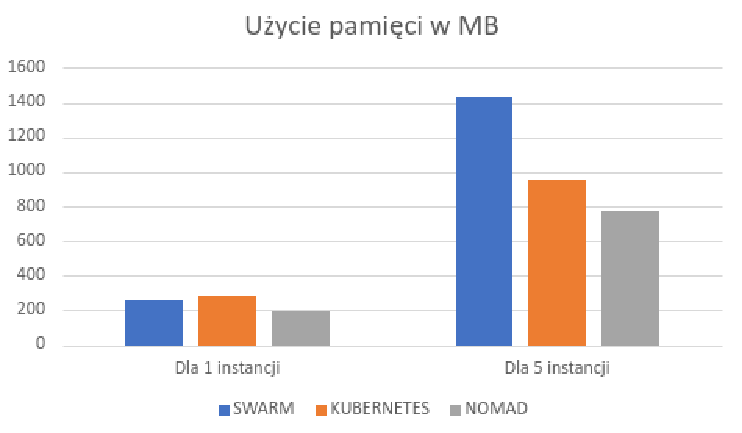
\includegraphics[width=12cm]{wynikiUzyciePamieci.pdf}
  \caption{Wyniki użycia pamięci dla aplikacji w orkiestratorach}
  \label{fig: Uzycie pamieci}
\end{figure}

Otrzymane wyniki użycia pamięci zostały ukazane na rysunku 
\ref{fig: Uzycie pamieci}. Użycie pamięci w przypadku jednej 
repliki aplikacji nieznacznie się różnią. Najlepszy wynik uzyskał 
Nomad, a najgorszy Kubernetes. Różnice się uwidaczniają 
w przypadku stworzenia nowych replik, gdzie najgorzej poradził 
sobie Docker Swarm, a wyniki dla Kubernetesa i Nomada nieznacznie 
się poprawiły w stosunku do wyników dla jednej repliki. Gdyby wymnożyć 
wynik dla 1 repliki razy 5 to wynik wyszedłby większy niż dla 
uruchomienia jednocześnie tych replik. Spowodowane jest to 
odpowiednim zarządzaniem zasobami. W dalszej częsci tego rozdziału 
zostały opisane techniki jakie stosuje każdy z orkiestatorów 
do rozdzielania zasobów i ich efektywnego wykorzystania.
\newline

\textbf{Quality of Service classes} - jest używane w przypadku 
\textbf{Kubernetesa} do klasyfikowania podów, które są uruchomione 
i alokowanie każdego poda w klasę QoS. Powoduje to, że pody są
różnie obsługiwane w zależności od tej klasyfikacji. Wynik tej 
klasyfikacji jest oparty na requestach kontenerów oraz czy został 
przekroczony limit zasobów. Klasy QoS są używane przez Kubernetesa 
do decydowania, które pody należy usunąć z węzła w którym występuje 
\textbf{Node Pressure}. Jest to proces w którym Kubelet usuwa 
pody, aby zwolnić używane przez nie zasoby.

W Kubernetesie są trzy rodzaje QoS. Kiedy Node będzie używał zasoby poza limitem w pierwszej 
kolejności uruchomi się \textbf{BestEffort}, następnie 
\textbf{Burstrable} oraz \textbf{Guaraneed}.

,,\textbf{Guaranteed}'' - pody w tym trybie mają z góry ustalony 
limit zasobów i są najmniej narażone na usunięcie. Mają 
gwarancję ich nie usuwania, aż do momentu przekroczenia 
limitów lub w przypadku, gdy nie będzie już podów o niższym 
priorytecie, które mogą zostać usunięte. Nie mogą uzyskać 
zasobów poza ustalonym w ich specyfikacji.

Kryteria jakie muszą spełniać pody, aby zaliczały się do tej 
kategorii:

\begin{itemize}
 \item zapytanie CPU musi być równe limitowi CPU każdego kontenera,
 \item każdy kontener musi mieć limit CPU i żądania CPU,
 \item zapytanie pamięci musi być równe limitowi pamięci każdego kontenera,
 \item każdy kontener musi mieć limit pamięci i żadania pamięci. 
\end{itemize}

Przykład:

\begin{lstlisting}[breaklines=true]

resources:
  requests:
    memory: "128Mi"
    cpu: "250m"
  limits:
    memory: "128Mi"
    cpu: "250m"

\end{lstlisting}


,,\textbf{Burstable}'' - pody w tym trybie mają ustalone 
minimalne gwarantowane zasoby bazujące na requescie, ale 
nie mają ustalonego górnego limitu. Zatem, jeśli limi nie jest 
sprecyzowany to domyślnie zasobami noda, więc odpowiedzalność 
za przydzielanie zasobów i zabierania ich spoczywa na nodzie i 
jego limicie. W przypadku, gdy node będzie chciał usunąć poda 
to będzie to mógł zrobić dopiero po wykonaniu \textbf{BestEffort}, 
ponieważ dany pod, który nie ma limitu może zabrać tyle zasobów 
ile będzie chciał.


Kryteria jakie muszą spełniać pody, aby zaliczały się do tej 
kategorii:

\begin{itemize}
 \item pod nie spełnia kryteriów, które charakteryzują klasę
 QoS \textbf{Guaranteed},
 \item przynajmniej jeden kontener w podzie musi mieć limit 
 pamięci albo CPU lub memory request albo cpu request,
\end{itemize}

Przykład: 

\begin{lstlisting}[breaklines=true]

resources:
  requests:
    memory: 100Mi
    cpu: 200m

\end{lstlisting}

,,\textbf{BestEffort}'' - pody w tej klasie mają dostęp do 
zasobów noda, które nie są przydzielone i używane przez inne 
pody. Jeśli wziąć na przykład procesor ryzen 5 5600x, który ma 
12 wątków i 4 wątki są juz przydzielone do podów. To pod w tej 
klasie może użyć pozostałych wolnych zasobów w nodzie. Pody 
w tej kategorii są najbardziej narażone na usunięcie w przypadku 
braku zasobów.

Pody w tej kategorii nie spełniają kryteriów tak jak 
w dwóch poprzednich kategoriach. Jeśli żaden kontener w podzie 
nie ma limitu pamięci lub limitu CPU, oraz nie ma zdefiniowanej 
pamięci oraz CPU na request to klasifikuje się jako BestEffort.

Dodatkowo kryteria, które zawsze muszą być zachowane bez 
względu na posiadana klasę: 

\begin{itemize}
  \item jak kontener przywłaszczy sobie zasobów poza ustalony 
  limit to zostanie usunięty i zrestartowany przez kubeleta bez 
  wpływu na inne kontenery,
  \item jeśli kontener przekroczy dane requesta i node na którym 
  działa ten kontener ma problemy z zasobami to taki kontener 
  jest kandydatem do usunięcia. Jeśli taka sytuacja się wydarze to 
  wszystkie kontenery w podzie będą zatrzymane i zostaną stworzone 
  zastępcze pody w innym nodzie,
  \item  zasoby requesta w podzie są równe sumie zasobów 
  requestów kontnerów w tym podzie. Co za tym idzie limit zasobów poda 
  jest równy sumie zasobów tworzących go kontenerów,
  \item kube-scheduler nie rozważa klas QoS podczas wyboru poda 
  do usunięcia.
\end{itemize}
 
Nomad nie posiada tak zaawansowanego systemu zarządzania zasobami, 
lecz także posiada kilka następujących procesów. Przy stwrzeniu 
nowego joba i przy jego zmianie lub błędzie Noda tworzony jest proces zwany 
\textbf{evaluation}, który jest przetwarzany przez evaluation brokera. 
Służy on do zarządzania kolejką z oczekujących \textbf{evaluation}. 
Odpowiednio zarządzą ich kolejnością i zapewnia, że wykonywany 
jest tylko jeden w tym samym czasie. Następnie 
\textbf{scheduling workers} uruchamiają odpowiedni scheduler 
na podstawie joba. Zadaniem \textbf{schedulera} jest wygenerowanie 
planu alokacji i analiza aktualnego stanu zasobów oraz potrzeby 
nodów. Za pomocą algorytmu takiego jak \textbf{bin packing} oraz 
reguł \textbf{anti-affinity} do optymalizacji zasobów. Ostatnim 
etapem zajmuje się \textbf{plan queue}, który podejmuje ostateczną 
decyzję.

\begin{figure}[!h]
  \centering
  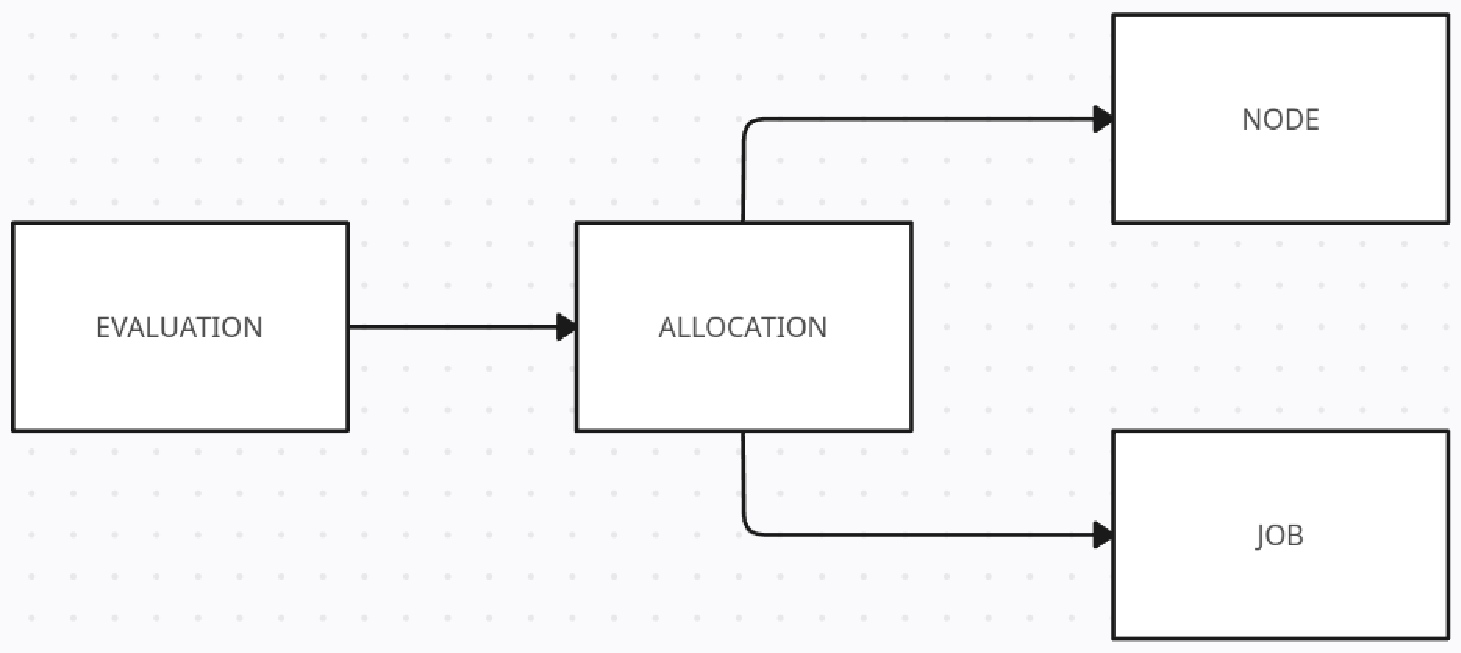
\includegraphics[width=12cm]{nomadalokacja.pdf}
  \caption{Alokacja zasobów Nomad}
  \label{fig: Alokacja zasobów Nomad}
\end{figure}

W nomadzie również można ustalić liczbę przedzielonych 
zasobów dla joba oraz ich maxymalna ilość.

\begin{lstlisting}[breaklines=true]

resources {
    cpu    = 100
    memory = 256
    memory_max = 512
}

\end{lstlisting}

Docker Swarm nie posiada algorytmu dla zarządzania zasobami 
serwisów, ale możliwe jest przypisanie wartości maksylanych 
i minialnych. Co nie jest wystarczające, aby uzyskać takie 
wyniki jakie posiadają wcześniej opisane orkiestratory.

\begin{lstlisting}[breaklines=true]

resources:
  limits:
    cpus: '0.50'   
    memory: '512M' 
  reservations:
    cpus: '0.25'   
    memory: '256M' 

\end{lstlisting}

\section{Wyniki i wnioski badania startu aplikacji}
\label{sec:StartAplikacji}

Wyniki dla czasu startu aplikacji w każdym z orkiestratorów 
można zobaczyć na rysunku \ref{fig: Czas startu aplikacji}. 
W przypadku jednej repliki wyniki dla Docker Swarma 
i Kubernetesa wyszły bardzo podobne (4,77s i 4,87s), a w przypadku 
Nomada wynik wyszedł troche lepszy (3,59s). Sytuacja się odwróciła 
w przypadku czasu uruchomieniu 5 aplikacji jednocześnie. 
Największy wzrost czasu przypadł Docker Swarmowi, bo aż 10,97s.
Spowodowane jest to brakiem zaawansowanych mechanizmów skalowania 
oraz słabsza optymalizacją zasobów. Najlepszy wynik uzyskał 
Kubernetes (5,154). Co jest wynikiem niewiele większym niż 
w przypadku jednej repliki. Możliwe jest to dzięki efektywnemu 
mechanizmowi zarządzania zasobami \textbf{QoS} opisanym 
w sekcji \ref{sec:Zarzadzanie zasobami}. Jak i również dzięki 
mechanizmowi wspomagającego tworzenie wiele aplikacji. 
Kubernetes posiada dwa takie mechanizmy, które nazywają się 
anti-affinity i pod affinity, które są zbiorem reguł pomagających 
określić, gdzie dany pod ma zostać umieszczony. Jest to coś 
podobnego do parametrów nodeSelectora, ale oferuje większą 
elastyczność i funkcjonalność. Nomad uzyskał wynik 5,31s. Jest 
to nieznacznie gorszy wynik niż w przypadku Kubernetesa. Taki 
wynik mógł uzyskać dzięki wykorzystaniu mechanizmów zarządzania 
zasobami takimi jak: \textbf{bin packing} 
oraz \textbf{memory max}. 

\begin{figure}[!h]
\centering
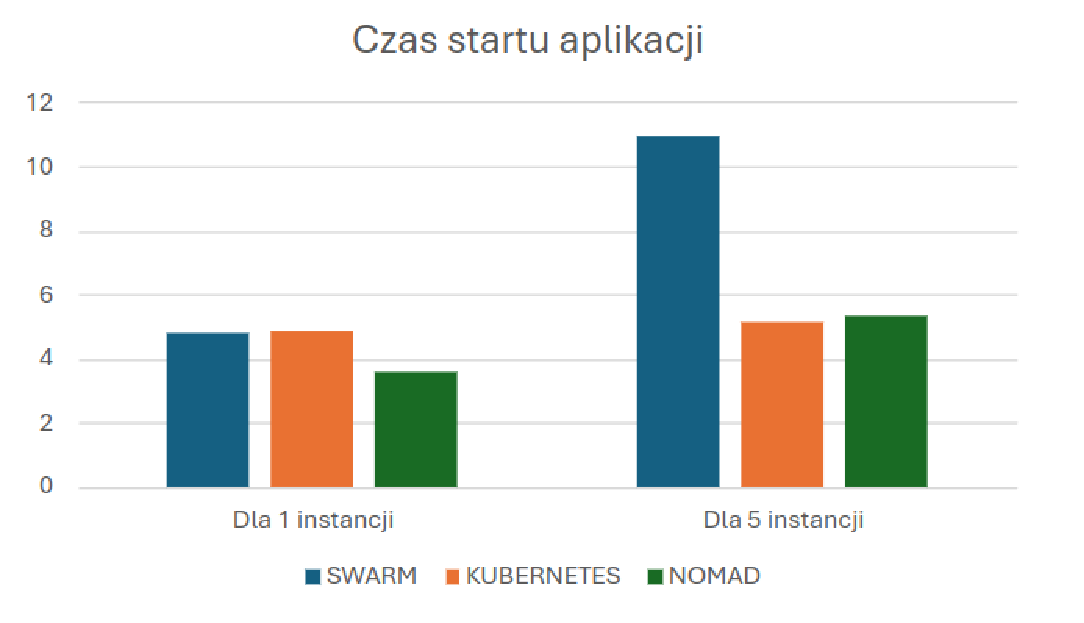
\includegraphics[width=12cm]{WynikiCzasStartu.pdf}
\caption{Czas startu aplikacji}
\label{fig: Czas startu aplikacji}
\end{figure}


\section{Wyniki i wnioski stabilności działania}

Test został przeprowadzony lokalnie. Wykorzystując 
\textbf{Keycloaka} wewnątrz \textbf{Dockera} przez co 
można było pominąć sytuacje chwilowego obiążenia tego 
narzędzia. Użytkownicy wysyłali zapytania do aplikacji, 
która potem pobierała dane z lokalnie zainstalowanej 
bazy danych i zwracała te dane. Po czym powinno się 
otrzymać prawidłowe dane oraz status.

Test polegał na wysłaniu określonej liczby zapytań 
w określonym czasie. W tym przypadku zostało wysłanych 
tyle zapytań, aż do momentu pojawienia się błędów. 

Najgorszy wynik uzyskał \textbf{Docker Swarm}, gdyż 
uzyskał jedynie 6000 pozytywnych \textbf{requestów} 
w czasie 30 sekund. Kubernetes uzyskał 21000 pozytywnych 
\textbf{requestów}, a najlepszy wynik uzyskał \textbf{Nomad},
bo aż 28000.

\begin{figure}[!h]
\centering
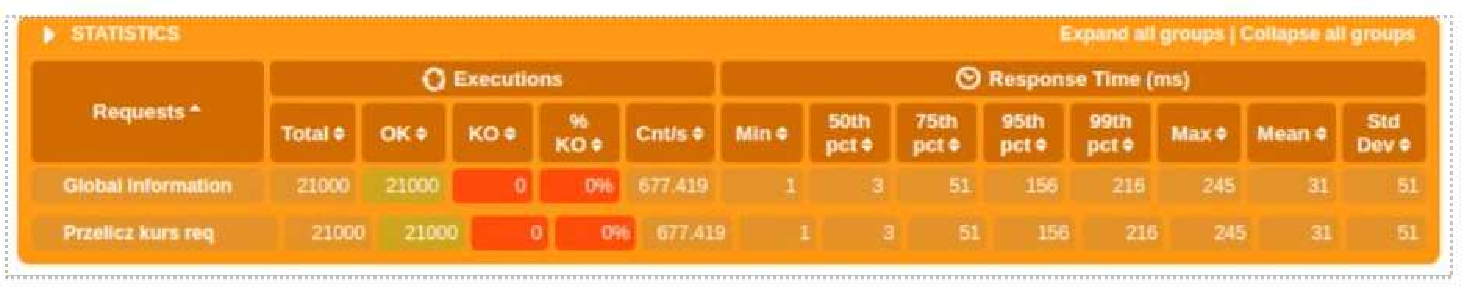
\includegraphics[width=12cm]{kubernetes/ObciazenieKubernetes.pdf}
\caption{Wynik działania narzędzia Gatling dla Kubernetesa}
\label{fig: Wynik działania narzędzia Gatling dla Kubernetesa}
\end{figure}

\begin{figure}[!h]
\centering
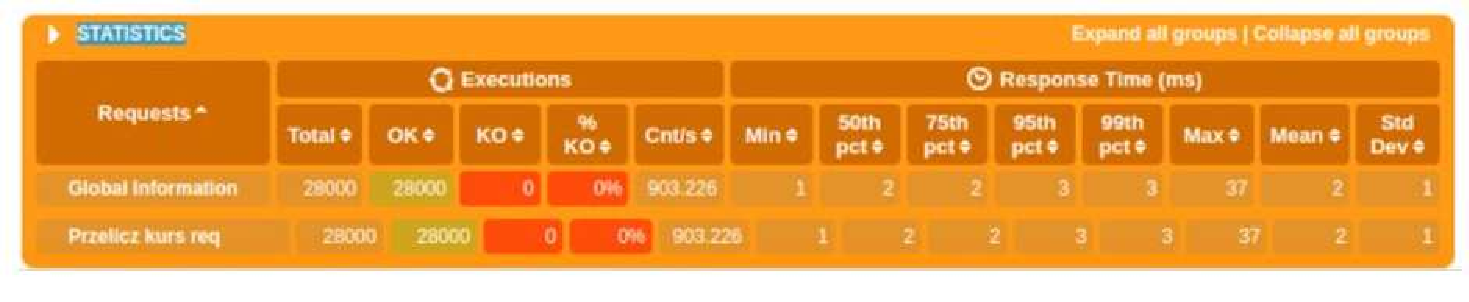
\includegraphics[width=12cm]{nomad/ObciazenieNomad.pdf}
\caption{Wynik działania narzędzia Gatling dla Nomada}
\label{fig: Wynik działania narzędzia Gatling dla Nomada}
\end{figure}

\begin{figure}[!h]
\centering
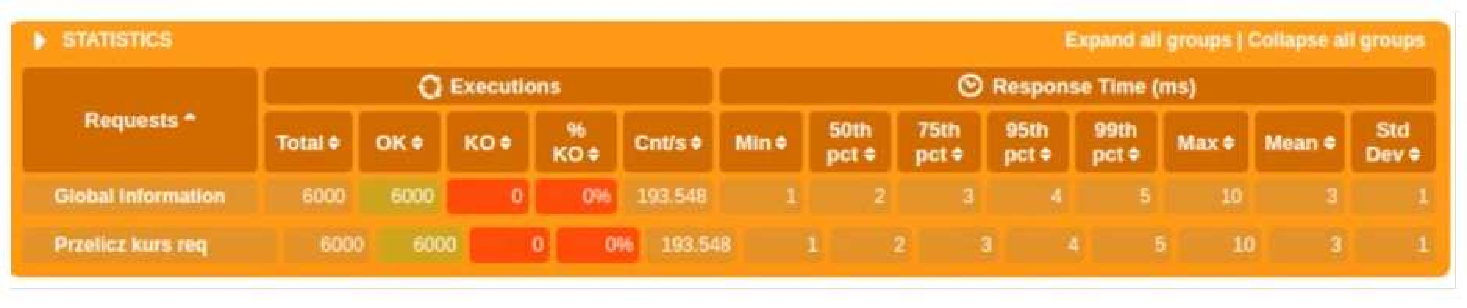
\includegraphics[width=12cm]{swarm/ObiazenieDockerSwarm.pdf}
\caption{Wynik działania narzędzia Gatling dla Docker Swarma}
\label{fig: Wynik działania narzędzia Gatling dla Docker Swarma}
\end{figure}

Obserwując użyte zasoby, można wywnioskować, że ilość udanych
wysłanych zapytań http ma swój limit w momencie przekroczenia 
przypisanej ilości pamięci ram. Na załączonym obrazku 
\ref{fig: Uzyte zasoby podczas testu Gatling} można zaobserwować 
skoki użycia procesora ponad limit 100MHz, lecz ilość użytej 
pamięci ram nie przekracza ustawionej granicy 300MiB. W momencie 
przekroczenia tej wartości job jest restartowany i kolejne 
requesty są bez odpowiedzi. 
Alokowanie pamięci nie jest dokładnie, ponieważ w przypadku 
aktualnego użycia pamięci na poziomie 150MiB/300MiB job 
pobierał ponad przy teście, a gdy aktualnie miał w użyciu 
ponad 250MiB (co mu wystarczało do obsłużenia zapytań) test 
przebiegał pomyślnie.

\begin{figure}[!h]
  \centering
  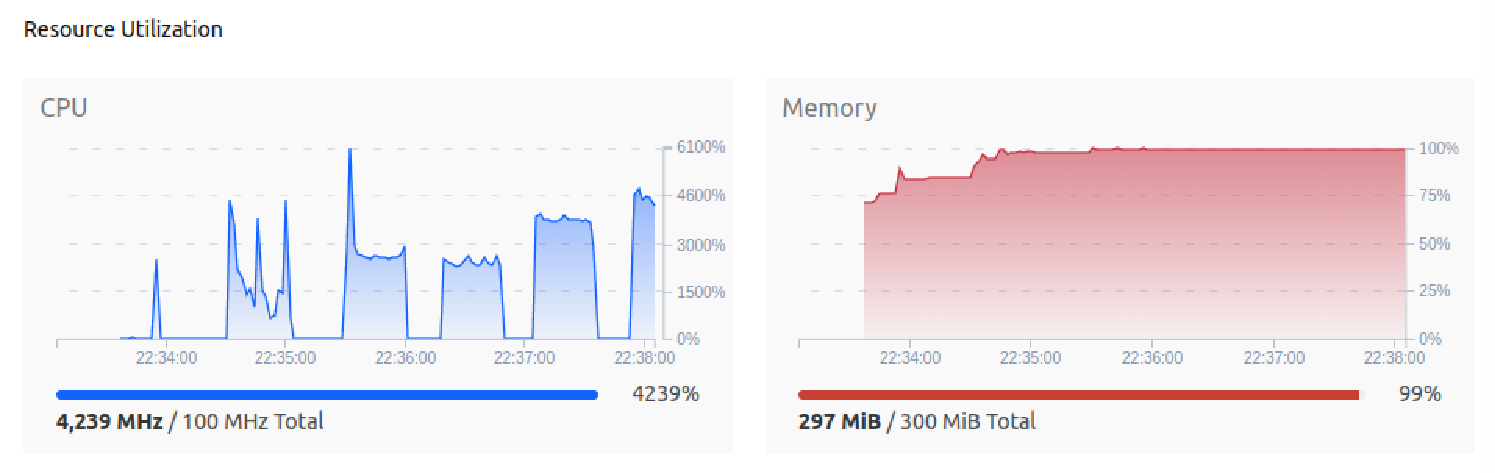
\includegraphics[width=12cm]{nomad/nomadGatlingTest.pdf}
  \caption{Użyte zasoby podczas testu Gatling}
  \label{fig: Uzyte zasoby podczas testu Gatling}
\end{figure}

%%%%%%%%%%%%%%%%%%%%%%%%%%%%%%%%%%%%%%%%%%%%%%%%%%%%%%%%%%%%%%%%
\cleardoublepage
\chapter*{Podsumowanie}
\label{cha:Podsumowanie}
\addcontentsline{toc}{chapter}{Podsumowanie}

% 1. Motywacja i kontekst

Motywacją podjęcia tematu analizy orkiestratorów było 
poznanie tych narzędzi z powodu coraz bardziej zwiększającego 
się zainteresowania tymi narzędziami w środowiskach komercyjnych. 
Są to narzędzia wspomagające pracę nad dużymi projektami, które 
znacznie ułatwiają organizację pracy nad nimi. Również programiści 
zaczęli przechodzić z tworzenia dużych monolitycznych aplikacji 
na aplikacje mikroserwisowe. Spowodowało to potrzebę wprowadzenia 
nowych rozwiązań pod ten typ. Szczegółowe różnice zostały opisane 
we wstępie w tabeli \ref{tab:Wady i zalety aplikacji Monolitycznych i mikroserwisowych}. 
W indywidualnych zadaniach programistycznych użycie ich mija się 
z celem, gdyż nie osiągają one takiej wielkości. Czas poświęcony na 
konfiguracje tych narzędzi będzie dużo większy, a korzyści z tego 
będą znikome. Podział aplikacji daje wiele korzyści w przypadku podziału 
zadań w zespole i łatwości w ustaleniu przyczyny błędów z powodu 
tworzenia aplikacji, gdzie jeden błąd nie ma tak dużego wpływu na resztę. 
Orkiestratory również wspomagają zarządzanie tymi aplikacjami poprzez 
mechanizmy takie jak automatyczna regeneracja. W obecnych czasach 
poznanie tych narzędzi jest argumentem do wejścia do nowoczesnych 
i dużych projektów.
\newline

% 2. Zakres pracy, przeprowadzone czynności (jasno wyszczególniony wkład wła-
% sny)

Celem pracy było zapoznanie się z narzędziami do orkiestracji 
kontenerów Docker. Poprzez przejrzenie literatury oraz dostępnych 
materiałów online. W pierwszej kolejności trzeba było sobie 
przypomnieć sposób działania Dockera i jego możliwości oraz komendy. 
Kolejnym krokiem było stworzenia aplikacji do testowania 
orkiestratorów oraz skonteneryzowania jej. Utworzona aplikacja 
opisana w rozdziale \ref{cha:Aplikacja} ma za zadanie pobranie danych 
z \url{https://api.nbp.pl/}. Zapisać te dane do bazy danych i na 
ich podstawie wykonać operacje CRUD. Dodatkową możliwościa jest 
kalkulator do przeliczenia jednej waluty na drugą przy pomocy kursów 
walut. Aplikacja została wykonana przy użyciu frameworka Quarkus. 
Pozwoliło to stworzyć aplikację już od samego początku przystosowaną 
do działania w kontenerze. Utworzony szablon zawierał instrukcję i plik 
za pomocą, którego został stworzony obraz. Aplikacja dodatkowo zawierała 
uwierztelnianie użytkownika za pomocą Keycloaka. Tak utworzona aplikację 
następnie została uruchomiona na każdym z orkiestratorów. Sposób 
uruchomienia został opisany w rozdziale \ref{cha:Orkiestratory}. 
Architektury w poszczególnych orkiestratorach zostały własnoręcznie 
opracowane i wdrożone lokalnie. Ostatnim etapem było przygotowanie 
testów do porównania orkiestratorów. Do przeprowadzenia testu 
sprawdzającego użyte zasoby zostały użyte narzędzia wbudowane 
oraz dockerswarm w przypadku Docker swarma. Test sprawdzający 
szybkość uruchomienia aplikacja, aż do momentu uzyskania prawidłowej 
odpowiedzi został napisany własnoręcznie w języku c. Ostatnim testem 
był test obiążenia wykonany przy użyciu narzędzia Gatling. Został 
napisany skrypt, którego zadaniem było wysyłanie określonej ilości 
zapytań w określonym czasie do aplikacji. 
\newline

% 3. Osiągnięte wyniki, interpretacja wyników, wnioski, etc.

Osiągnięte wyniki częściowo pokrywały się z~przewidywanymi jeszcze 
przed rozpoczęciem testowania. Najgorsze wyniki w przypadku jednej 
instancji uzyskał Kubernetes. Spowodowane jest to przez samo rozbudowanie 
orkiestratora. Posiada on wiele funkcji, które sa zoptymalizowane pod 
działanie przy wielu replikach i kontenerach. Dodatkowo wymaga 
zainstalowania i urucomienie klastra w kontenerze, co powoduje 
dodatkowy narzut na wydajność. Drugie w kolejności wyniki dla 
jednej repliki uzyskał Docker Swarm z powodu tego, że jest 
to narzędzie wbudowane do Dockera. Ma również najprostszą budowę 
i małą ilość funkcji. Najlepsze wyniki osiągnął Nomad dla jednej 
repliki. W przypadku testów dla wielu replik najlepsze wyniki uzyskał 
Kubernetes. Można było zauważyc działające mechanizm, które 
zoptymalizowały wykonywane operacje. Za pomocą mechanik takim 
jak QoS, którego celem jest inteligente zarządzanie zasobami.
Pozwoliło mu w teście na użycie zasobów uzyskać wynik, który nie jest 
wielokrotnością wyniku dla jednej instancji. W kolejnym teście 
na czas startu instancji uzyskał on wynik dla 5 instancji 
prawie identyczny jak w przypadku jednej instacji 
anty-affinity i affinity pozwalającymi określić miejsce umieszczenie 
podów w nodzie. Najgorzej skalował się Docker Swarm, gdyż nie posiada 
w sobie zaiplementowanych zaawansowanych mechanizmów kontroli nad 
zasobami. Istnieje tylko mozliwość podania na sztywno tych danych. 
Nomad wypadł gorzej od Kubernetesa, ale lepiej od Docker Swarma. 
Można było zauważyc pewne mechaizmy jak bin-packing, które wpłynęły 
na ilość użytych zasobów przy zwiększeniu liczby instancji.

Docker Swarm mimo, że nie posiada zaawansowanych mechanizmów to 
idealnie sprawdzi się w mniej skomplikowanych wdrożeniach 
i w zespołach mniej doświadczonych osób, gdyż jest prosty 
w obsłudze oraz jest zintegrowany z Dockerem. Jest to również 
narzędzie bezpłatne, więc można od niego rozpocząć zaznajamianie 
się z tematyką orkiestracji.

Zaawansowane funkcje Kubernetesa idealnie sprawdzą się przy dużych 
i złożonych projektach, które wymagają jak największej wydajności 
i kontroli oraz wysokiej skalowalności. Co pokazują uzyskane wyniki 
testów. Wykorzystany w pracy klaster Kubernetesa Minikube jest 
rozwiązaniem, które powinno się używać wyłącznie do testów lokalnie. 
Nie posiada on wszystkich funkcji dostępnych w Kubernetesie. 
Korzystanie z Kubernetesa w chymrze obarczone jest kosztami za 
zasoby obliczeniowe, pamięć, sięć oraz dodatkowe usługi jak 
w AWS albo Azure.

Nomad może mieć zastosowanie tam, gdzie wymagana jest lekka 
architektura i efektywne zarządzanie zasobami. Warto go rozważyć 
w organizacjach, które mają ograniczony budżet i zasoby. Nomad 
podobnie jak Kubernetes ma opcję używania go bezpłanie oraz 
możliwość płatnego dostępu w celu używania go w chmurze. Jest 
także możliwość wykupienia wersji Enterprise oprogramowania, która 
zawiera funkcje niedostępne w zwykłej wersji.
\newline

% 4. Ocena spełnienia założeń i osiągnięcia celu pracy

Ostatecznie udało się stworzyć aplikację i ją skonteneryzować. 
Skonfigurować orkiestratory i wdrożyć aplikację do każdego z nich. 
Aplikacja działała tak jak było to oczekiwane. Wdrożenie aplikacji 
na orkiestratory było takie samo. Z tą różnica, że każdy z nich 
składa się z innych elementów. 
Wyniki dla obciążenia procesora nie pokazywały różnic z powodu, że 
różne narzędzia wskazywały różne jednostki. Przez co nie można było 
wyciągnać żadnych wniosków. Wyniki dla pozostałych testów wyszły 
poprawne. Można było wyciągnać z nich wnioski i zauważyc różnice 
w zastosowanych rozwiązaniach i użytych mechanizmów.
\newline

% 5. Perspektywy rozwoju

W dalszej perspektywie można rozważyć użycie jednego narzędzia do 
sprawdzenia obciążenia podzespołow. Przykładem takiego narzędzia 
może być Prometheus w połączeniu z Graphaną. 

Można również bardziej rozbudować architekturę aplikacji. Dodając do niej kolejne serwisy, 
np. część kliencką aplikacji. Pozwalającą użytkownikowi używać 
aplikacji przy pomocy interfejsu graficznego w przeglądarce. W ten 
sposób można stworzyć architekturę zbliżona do tych, które tworzy 
się w komercyjnych projektach.

Kolejną opcją może być analiza kosztów w przypadku używania 
orkiestratorów w chmurze.


% dołączenie bibliografii z~pliku biblio.bib (tylko pozycje odwołane w~tekście, zgodnie z~formatowaniem ,,unsrt'' - numerowane kolejnością wystąpienia)
\cleardoublepage
\addcontentsline{toc}{chapter}{Bibliografia}
\bibliography{biblio}
\bibliographystyle{unsrt}

%Spis rysunków
%\newpage
\listoffigures

%Spis tabel
%\newpage
\listoftables

\end{document}
